  %%% آپدیت شده در شهریور 1402

%%% مواردی که نسبت به قبل بروزرسانی شده است به شرح زیر می باشد
%%% 1- بولد شدن سر فصل ها
%%% 2- اضافه شدن قابلیت
%%%    \begin{subfigure}
%%% 3-   اصلاح ترتیب شماره گذاری مراجع به ترتیب اولویت ارجاع در متن 
%%% 4- مرتب شدن فایل‌ها (قرار گرفتن عکس ها و فونت ها در پوشه ای جداگانه)
%%% 5- اضافه شدن پکیج فرض
%%% 6- اضافه شدن فونت یاس برای فارسی شدن اعداد
%%% 7- اضافه شدن پکیج تنظیم سایز جدول


%%%  کلاس AUTthesis، نسخه آبان 1397
%%%   دانشگاه صنعتی امیرکبیر                 http://www.aut.ac.ir
%%%  تالار گفتگوی پارسی‌لاتک،       http://forum.parsilatex.com
%%%   آپدیت شده در آبان 95
%%%   پشتیبانی و راهنمایی          badali_farhad@yahoo.com
%%%
%%%   بازبینی و اصلاح شده در آبان ماه 1397
%%%  Tested via TeXstudio in TeXlive 2014-2018.
%%%

%-----------------------------------------------------------------------------------------------------
%        روش اجرا.: 2 بار F1 ، 2 بار  F11(به منظور تولید مراجع) ، دوبار Ctrl+Alt+I (به منظور تولید نمایه) و دو بار F1 -------> مشاهده Pdf
%%%%%%%%%%%%%%%%%%%%%%%%%%%%%%%%%%%%%%%%%%%%%%%%%%%%%%
%   TeXstudio as your IDE
%%  برای compile در TeXstudio تنها کافی است منوی Options->Configure TeXstudio را زده و در پنجره Configure TeXstudio در بخش Build گزینه Default Compiler را به XeLaTeX تغییر دهید. سند شما به راحتی compile خواهد شد.
%   F1 & F5 : Build & view
%   F6      : Compile
%   F7      : View
%   --------------
%%%%%%%%%%%%%%%%%%%%%%%%%%%%%%%%%%%%%%%%%%%%%%%%%%%%%%
%        اگر قصد نوشتن رساله دکتری را دارید، در خط زیر به جای msc،
%      کلمه phd را قرار دهید. کلیه تنظیمات لازم، به طور خودکار، اعمال می‌شود.
%%% !TEX TS-program = XeLaTeX
\documentclass[oneside,msc,12pt]{AUTthesis}
%       فایل commands.tex را حتماً به دقت مطالعه کنید؛ چون دستورات مربوط به فراخوانی بسته زی‌پرشین 
%       و دیگر بسته‌ها و ... در این فایل قرار دارد و بهتر است که با نحوه استفاده از آنها آشنا شوید. توجه شود برای نسخه نهایی پایان‌نامه حتماً hyperref را 
%        غیرفعال کنید.


% در این فایل، دستورها و تنظیمات مورد نیاز، آورده شده است.
%-------------------------------------------------------------------------------------------------------------------
% در ورژن جدید زی‌پرشین برای تایپ متن‌های ریاضی، این سه بسته، حتماً باید فراخوانی شود.
\usepackage{amsthm,amssymb,amsmath,amsfonts}
% بسته‌ای برای تنطیم حاشیه‌های بالا، پایین، چپ و راست صفحه
\usepackage[top=30mm, bottom=30mm, left=25mm, right=30mm]{geometry}
% بسته‌‌ای برای ظاهر شدن شکل‌ها و تصاویر متن
\usepackage{graphicx}
\usepackage{color}
%بسته‌ای برای تنظیم فاصله عمودی خط‌های متن
\usepackage{setspace}
\usepackage{titletoc}
\usepackage{tocloft}
%با فعال کردن بسته زیر فوت‌نوت‌ها در هر صفحه ریست می‌شوند. حالت پیش‌فرض آن ریست شدن در هر فصل می‌باشد.
%\usepackage[perpage]{footmisc}
\usepackage{enumitem}
\usepackage{multirow,adjustbox}
%\usepackage{titlesec}
% بسته‌ و دستوراتی برای ایجاد لینک‌های رنگی با امکان جهش
\usepackage[pagebackref=false,colorlinks,linkcolor=blue,citecolor=red]{hyperref}
\usepackage[nameinlink]{cleveref}%capitalize,,noabbrev
\AtBeginDocument{%
	\crefname{equation}{برابری}{equations}%
	\crefname{chapter}{فصل}{chapters}%
	\crefname{section}{بخش}{sections}%
	\crefname{appendix}{پیوست}{appendices}%
	\crefname{enumi}{مورد}{items}%
	\crefname{footnote}{زیرنویس}{footnotes}%
	\crefname{figure}{شکل}{figures}%
	\crefname{table}{جدول}{tables}%
	\crefname{theorem}{قضیه}{theorems}%
	\crefname{lemma}{لم}{lemmas}%
	\crefname{corollary}{نتیجه}{corollaries}%
	\crefname{proposition}{گزاره}{propositions}%
	\crefname{definition}{تعریف}{definitions}%
	\crefname{result}{نتیجه}{results}%
	\crefname{example}{مثال}{examples}%
	\crefname{remark}{نکته}{remarks}%
	\crefname{note}{یادداشت}{notes}%
    \crefname{asum}{فرض}{Assumption}
	% دستوری برای تغییر نام کلمه «کتاب‌نامه» به «منابع و مراجع«
	\renewcommand{\bibname}{منابع و مراجع}

    \renewcommand{\labelitemi}{$\bullet$}
    % دستوری برای تعیین علامت سطح دوم itemize
    \renewcommand{\labelitemii}{$\circ$}
    % دستوری برای تعیین علامت سطح سوم itemize
    \renewcommand{\labelitemiii}{$-$}
    % برای سطح چهارم
    \renewcommand{\labelitemiv}{$*$}
    % دستوری برای تغییر نام کلمه «اثبات» به «برهان»
    \renewcommand\proofname{\textbf{برهان}}
    \renewcommand{\listfigurename}{فهرست شکل‌ها}
    \renewcommand{\listtablename}{فهرست جدول‌ها}
}

\usepackage{subcaption}
% چنانچه قصد پرینت گرفتن نوشته خود را دارید، خط بالا را غیرفعال و  از دستور زیر استفاده کنید چون در صورت استفاده از دستور زیر‌‌، 
% لینک‌ها به رنگ سیاه ظاهر خواهند شد که برای پرینت گرفتن، مناسب‌تر است
%\usepackage[pagebackref=false]{hyperref}
% بسته‌ لازم برای تنظیم سربرگ‌ها
\usepackage{fancyhdr}
% بسته‌ای برای ظاهر شدن «مراجع»  در فهرست مطالب
\usepackage[nottoc]{tocbibind}
% دستورات مربوط به ایجاد نمایه
\usepackage{makeidx,multicol}
\setlength{\columnsep}{1.5cm}

%%%%%%%%%%%%%%%%%%%%%%%%%%
\usepackage{verbatim}
\makeindex
\usepackage{sectsty}
% فراخوانی بسته زی‌پرشین و تعریف قلم فارسی و انگلیسی
\usepackage{xepersian}%[extrafootnotefeatures]
\SepMark{-}
%حتماً از تک لایو 2014 استفاده کنید.
\settextfont[Scale=1.2,Path=Fonts/,BoldFont=B Nazanin Bold.ttf]{B Nazanin.ttf}
\setlatintextfont[Path=Fonts/,BoldFont=timesbd]{times}

%%%%%%%%%%%%%%%%%%%%%%%%%%
% چنانچه می‌خواهید اعداد در فرمول‌ها، انگلیسی باشد، خط زیر را غیرفعال کنید.
%
%\setdigitfont[Scale=1.1]{PGaramond}%%Yas
%%%%%%%%%%%%%%%%%%%%%%%%%%
% تعریف قلم‌های فارسی اضافی برای استفاده در بعضی از قسمت‌های متن
\defpersianfont\nastaliq[Scale=2,Path=Fonts/]{IranNastaliq.ttf}
\defpersianfont\chapternumber[Scale=3,Path=Fonts/,BoldFont=B Nazanin Bold.ttf]{B Nazanin.ttf}
%\chapterfont{\centering}%
%%%%%%%%%%%%%%%%%%%%%%%%%%





% Headings for every page of ToC, LoF and Lot
\setlength{\cftbeforetoctitleskip}{-1.2em}
\setlength{\cftbeforelottitleskip}{-1.2em}
\setlength{\cftbeforeloftitleskip}{-1.2em}
\setlength{\cftaftertoctitleskip}{-1em}
\setlength{\cftafterlottitleskip}{-1em}
\setlength{\cftafterloftitleskip}{-1em}
%%\makeatletter
%%%%\renewcommand{\l@chapter}{\@dottedtocline{1}{1em\bfseries}{1em}}
%%%%\renewcommand{\l@section}{\@dottedtocline{2}{2em}{2em}}
%%%%\renewcommand{\l@subsection}{\@dottedtocline{3}{3em}{3em}}
%%%%\renewcommand{\l@subsubsection}{\@dottedtocline{4}{4em}{4em}}
%%%%\makeatother


\newcommand\tocheading{\par عنوان\hfill صفحه \par}
\newcommand\lofheading{\hspace*{.5cm}\figurename\hfill صفحه \par}
\newcommand\lotheading{\hspace*{.5cm}\tablename\hfill صفحه \par}

\renewcommand{\cftchapleader}{\cftdotfill{\cftdotsep}}
\renewcommand{\cfttoctitlefont}{\hspace*{\fill}\LARGE\bfseries}%\Large
\renewcommand{\cftaftertoctitle}{\hspace*{\fill}}
\renewcommand{\cftlottitlefont}{\hspace*{\fill}\LARGE\bfseries}%\Large
\renewcommand{\cftafterlottitle}{\hspace*{\fill}}
\renewcommand{\cftloftitlefont}{\hspace*{\fill}\LARGE\bfseries}
\renewcommand{\cftafterloftitle}{\hspace*{\fill}}

%%%%%%%%%%%%%%%%%%%%%%%%%%
% تعریف و نحوه ظاهر شدن عنوان قضیه‌ها، تعریف‌ها، مثال‌ها و ...
%برای شماره گذاری سه تایی قضیه ها
\theoremstyle{definition}
\newtheorem{definition}{تعریف}[section]
\newtheorem{remark}[definition]{نکته}
\newtheorem{note}[definition]{یادداشت}
\newtheorem{example}[definition]{نمونه}
\newtheorem{question}[definition]{سوال}
\newtheorem{remember}[definition]{یاداوری}
\theoremstyle{theorem}
\newtheorem{theorem}[definition]{قضیه}
\newtheorem{lemma}[definition]{لم}
\newtheorem{proposition}[definition]{گزاره}
\newtheorem{corollary}[definition]{نتیجه}
\newtheorem{asum}[definition]{فرض}
%%%%%%%%%%%%%%%%%%%%%%%%
%%%%%%%%%%%%%%%%%%%
%%% برای شماره گذاری چهارتایی قضیه ها و ...
%%\newtheorem{definition1}[subsubsection]{تعریف}
%%\newtheorem{theorem1}[subsubsection]{قضیه}
%%\newtheorem{lemma1}[subsubsection]{لم}
%%\newtheorem{proposition1}[subsubsection]{گزاره}
%%\newtheorem{corollary1}[subsubsection]{نتیجه}
%%\newtheorem{remark1}[subsubsection]{نکته}
%%\newtheorem{example1}[subsubsection]{مثال}
%%\newtheorem{question1}[subsubsection]{سوال}

%%%%%%%%%%%%%%%%%%%%%%%%%%%%

% دستورهایی برای سفارشی کردن صفحات اول فصل‌ها
\makeatletter
\newcommand\mycustomraggedright{%
	\if@RTL\raggedleft%
	\else\raggedright%
	\fi}
\def\@makechapterhead#1{%
	\thispagestyle{style1}
	\vspace*{20\p@}%
	{\parindent \z@ \mycustomraggedright
		\ifnum \c@secnumdepth >\m@ne
		\if@mainmatter
		
		\bfseries{\Huge \@chapapp}\small\space {\chapternumber\thechapter}
		\par\nobreak
		\vskip 0\p@
		\fi
		\fi
		\interlinepenalty\@M 
		\Huge \bfseries #1\par\nobreak
		\vskip 120\p@
		
	}
	
	%\thispagestyle{empty}
	\newpage}
\bidi@patchcmd{\@makechapterhead}{\thechapter}{\tartibi{chapter}}{}{}
\bidi@patchcmd{\chaptermark}{\thechapter}{\tartibi{chapter}}{}{}
\makeatother

\pagestyle{fancy}
\renewcommand{\chaptermark}[1]{\markboth{\chaptername~\tartibi{chapter}: #1}{}}

\fancypagestyle{style1}{
	\fancyhf{} 
	\fancyfoot[c]{\thepage}
	\fancyhead[R]{\leftmark}%
	\renewcommand{\headrulewidth}{1.2pt}
}


\fancypagestyle{style2}{
	\fancyhf{}
	\fancyhead[R]{چکیده}
	\fancyfoot[C]{\thepage{}}
	\renewcommand{\headrulewidth}{1.2pt}
}

\fancypagestyle{style3}{%
	\fancyhf{}%
	\fancyhead[R]{فهرست نمادها}
	\fancyfoot[C]{\thepage}%
	\renewcommand{\headrulewidth}{1.2pt}%
}

\fancypagestyle{style4}{%
	\fancyhf{}%
	\fancyhead[R]{فهرست جدول‌ها}
	\fancyfoot[C]{\thepage}%
	\renewcommand{\headrulewidth}{1.2pt}%
}

\fancypagestyle{style5}{%
	\fancyhf{}%
	\fancyhead[R]{فهرست شکل‌ها}
	\fancyfoot[C]{\thepage}%
	\renewcommand{\headrulewidth}{1.2pt}%
}

\fancypagestyle{style6}{%
	\fancyhf{}%
	\fancyhead[R]{فهرست مطالب}
	\fancyfoot[C]{\thepage}%
	\renewcommand{\headrulewidth}{1.2pt}%
}

\fancypagestyle{style7}{%
	\fancyhf{}%
	\fancyhead[R]{نمایه}
	\fancyfoot[C]{\thepage}%
	\renewcommand{\headrulewidth}{1.2pt}%
}

\fancypagestyle{style8}{%
	\fancyhf{}%
	\fancyhead[R]{منابع و مراجع}
	\fancyfoot[C]{\thepage}%
	\renewcommand{\headrulewidth}{1.2pt}%
}
\fancypagestyle{style9}{%
	\fancyhf{}%
	\fancyhead[R]{واژه‌نامه‌ی فارسی به انگلیسی}
	\fancyfoot[C]{\thepage}%
	\renewcommand{\headrulewidth}{1.2pt}%
}
%


%دستور حذف نام لیست تصاویر و لیست جداول از فهرست مطالب
\newcommand*{\BeginNoToc}{%
	\addtocontents{toc}{%
		\edef\protect\SavedTocDepth{\protect\the\protect\value{tocdepth}}%
	}%
	\addtocontents{toc}{%
		\protect\setcounter{tocdepth}{-10}%
	}%
}
\newcommand*{\EndNoToc}{%
	\addtocontents{toc}{%
		\protect\setcounter{tocdepth}{\protect\SavedTocDepth}%
	}%
}
\newcounter{savepage}

%\renewcommand\cftsecleader{\cftdotfill{\cftdotsep}}
%%%%%%%%%%%%%%%%%%%%%%%%%%%%%
%%%%%%%%%%%%%%%%%%%%%%%%%%%%

\begin{document}
\baselineskip=.75cm
\linespread{1.75}
%% -!TEX root = AUTthesis.tex
% در این فایل، عنوان پایان‌نامه، مشخصات خود، متن تقدیمی‌، ستایش، سپاس‌گزاری و چکیده پایان‌نامه را به فارسی، وارد کنید.
% توجه داشته باشید که جدول حاوی مشخصات پروژه/پایان‌نامه/رساله و همچنین، مشخصات داخل آن، به طور خودکار، درج می‌شود.
%%%%%%%%%%%%%%%%%%%%%%%%%%%%%%%%%%%%
% دانشکده، آموزشکده و یا پژوهشکده  خود را وارد کنید
\faculty{دانشکده ...}
% گرایش و گروه آموزشی خود را وارد کنید
\department{گرایش ...}
% عنوان پایان‌نامه را وارد کنید
\fatitle{عنوان پایان نامه-دستورالعمل و راهنمای نگارش
\\[.75 cm]
 پایان‌نامه}
% نام استاد(ان) راهنما را وارد کنید
\firstsupervisor{نام کامل استاد راهنما}
%\secondsupervisor{استاد راهنمای دوم}
% نام استاد(دان) مشاور را وارد کنید. چنانچه استاد مشاور ندارید، دستور پایین را غیرفعال کنید.
\firstadvisor{نام کامل استاد مشاور}
%\secondadvisor{استاد مشاور دوم}
% نام نویسنده را وارد کنید
\name{نام }
% نام خانوادگی نویسنده را وارد کنید
\surname{و نام خانوادگی کامل نویسنده}
%%%%%%%%%%%%%%%%%%%%%%%%%%%%%%%%%%
\thesisdate{ماه و سال}

% چکیده پایان‌نامه را وارد کنید
\fa-abstract{
در اين قسمت چكيده پایان نامه نوشته مي‌شو‌د‌.‌ چكيده بايد جامع و بيان‌كننده‌ خلاصه‌اي از اقدامات انجام‌شده باشد. در چكيده باید از ارجاع به مرجع و ذكر روابط رياضي، بيان تاريخچه و تعريف مسئله خودداري ‌شود. 
}


% کلمات کلیدی پایان‌نامه را وارد کنید
\keywords{کلیدواژه اول، ...، کلیدواژه پنجم (نوشتن سه تا پنج واژه کلیدی ضروری است)}



\AUTtitle
%%%%%%%%%%%%%%%%%%%%%%%%%%%%%%%%%%
\vspace*{7cm}
\thispagestyle{empty}
\begin{center}

\includegraphics[height=5cm,width=12cm]{Images/besm.jpg}
\end{center}
% تاییدیه دفاع
\newpage
\thispagestyle{empty}
%\fontsize{18pt}{19pt}\selectfont

\section*{صفحه فرم ارزیابی و تصویب پایان نامه- فرم تأیید اعضاء كميته دفاع}

\fontsize{12pt}{14pt}\selectfont
%\renewcommand{\baselinestretch}{1.5}
\vspace*{1cm}
   در این صفحه فرم دفاع یا تایید و تصویب پایان نامه موسوم به فرم کمیته دفاع- موجود در پرونده آموزشی- را قرار دهید.
\vspace*{1cm}


\subsection*{نکات مهم:}
 
\begin{itemize}
\item
	نگارش پایان نامه/رساله باید به
	{\color{red}
		زبان فارسی
	}
	و بر اساس آخرین نسخه دستورالعمل و راهنمای تدوین پایان نامه های دانشگاه صنعتی امیرکبیر باشد.(دستورالعمل و راهنمای حاضر)
\item رنگ جلد پایان نامه/رساله چاپي كارشناسي، كارشناسي ارشد و دكترا  بايد به ترتيب مشكي، طوسي و سفيد رنگ باشد.  
\item چاپ و صحافی پایان نامه/رساله بصورت
{\color{red}
	پشت و رو(دورو)
}
بلامانع است و انجام آن توصيه مي شود. 
\end{itemize}
%%%%%%%%%%%%%%%%%%%%%%%%%%%%%%%%%%%%%%%%%%%%%%%%%%%%%%%%%%%%%%%%%%%%%%%%%%%%%%%%%%%%%%%%%%%%%%%%%%
%%%%%%%%%%%%%%%%%%%%%%%%%%%%%%%%%%%%%%%%%%%%%%%%%%%%%%%%%%%%%%%%%%%%%%%%%%%%%%%%%%%%%%%%%%%%%%%%%%
\newpage
\thispagestyle{empty}
\begin{picture}(50,50)
  \put(17,0){
\includegraphics[scale=1.1]{fa-logo.png}}
  \put(4.5,-13){\footnotesize{دانشگاه صنعتی امیرکبیر}}
  \put(10.5,-27){\footnotesize{(پلی‌تکنیک تهران)}}
  \put(170,30){\bf{به نام خدا}}
  \put(140,-5){\Large\bf{تعهدنامه اصالت اثر}}
  \put(310,0){تاریخ: \datethesis}
\end{picture}

\vspace*{2.5cm}

اينجانب {\bf{\fname\lname}} متعهد می‌شوم که مطالب مندرج در این پایان‌نامه حاصل کار پژوهشی اینجانب تحت نظارت و راهنمایی اساتید دانشگاه صنعتی امیرکبیر بوده و به دستاوردهای دیگران که در این پژوهش از آنها استفاده شده است مطابق مقررات و روال متعارف ارجاع و در فهرست منابع و مآخذ ذکر گردیده است. این پایان‌نامه قبلاً برای احراز هیچ مدرک هم‌سطح یا بالاتر ارائه نگردیده است.

در صورت اثبات تخلف در هر زمان، مدرک تحصیلی صادر شده توسط دانشگاه از درجه اعتبار ساقط بوده و دانشگاه حق پیگیری قانونی خواهد داشت.


کلیه نتایج و حقوق حاصل از این پایان‌نامه متعلق به دانشگاه صنعتی امیرکبیر می‌باشد. هرگونه استفاده از نتایج علمی و عملی، واگذاری اطلاعات به دیگران یا چاپ و تکثیر، نسخه‌برداری، ترجمه و اقتباس از این پایان نامه بدون موافقت کتبی دانشگاه صنعتی امیرکبیر ممنوع است. 
نقل مطالب با ذکر مآخذ بلامانع است.\\
\vspace{2.5cm}


{\centerline {\bf{\fname\lname}}}
\vspace*{.2cm}
{{\signature}}

%%%%%%%%%%%%%%%%%%%%%%%%%%%%%%%%%
% چنانچه مایل به چاپ صفحات «تقدیم»، «نیایش» و «سپاس‌گزاری» در خروجی نیستید، خط‌های زیر را با گذاشتن ٪  در ابتدای آنها غیرفعال کنید.
% پایان‌نامه خود را تقدیم کنید
% نیایش خود را در فایل زیر بنویسید.
\begin{acknowledgementpage}

\vspace{1.5cm}

{\nastaliq
{
 نويسنده پايان‌نامه، درصورت تمايل ميتواند برای سپاسگزاری پايان‌نامه خود را به شخص يا اشخاص و يا ارگان خاصی تقدیم نماید.
}}\end{acknowledgementpage}
\newpage
% سپاسگزاری را در فایل زیر بنویسید.
%%%%%%%%%%%%%%%%%%%%%%%%%%%%%%%%%%%%
\newpage\thispagestyle{empty}
% سپاس‌گزاری
{\nastaliq
سپاس‌گزاری
}
\\[2cm]

 نويسنده پايان‌نامه می‌تواند مراتب امتنان خود را نسبت به استاد راهنما و استاد مشاور و یا ديگر افرادي كه طي انجام پايان‌نامه به نحوي او را یاری و یا با او همكاری نموده‌اند ابراز دارد.














% با استفاده از دستور زیر، امضای شما، به طور خودکار، درج می‌شود.
\signature








%%%%%%%%%%%%%%%%%%%%%%%%%%%%%%%%%%%%%%%%%
%%%%%%%%%%%%%%%%%%%%%%%%%%%%%%%%%کدهای زیر را تغییر ندهید.
\newpage\clearpage

\pagestyle{style2}

\vspace*{-1cm}
\section*{\centering چکیده}
%\addcontentsline{toc}{chapter}{چکیده}
\vspace*{.5cm}
\ffa-abstract
\vspace*{2cm}


{\noindent\large\textbf{واژه‌های کلیدی:}}\par
\vspace*{.5cm}
\fkeywords
% دستور زیر برای شماره گذاری صفحات قبل از فصل اول با حروف ابجد است.
\pagenumbering{alph}
%-----------------------------------------------------------------------------
% فایل زیر دستورات مربوط به نمایش صفحات فهرست مطالب- فهرست اشکال و جداول است.
%{\pagestyle{style2}
%\tableofcontents}\newpage
%
%\listoffigures
\cleardoublepage
\pagestyle{style6}
\tableofcontents
\pagestyle{style6}
\cleardoublepage
%اگر لیست تصاویر و لیست جداول ندارید ، کدهای زیر را با گذاشتن % در ابتدای آنها، غیرفعال کنید.
\BeginNoToc
%============
\addtocontents{lof}{\lofheading}% add heading to the first page in LoF
\pagestyle{style5}
\listoffigures
\thispagestyle{style5}
\cleardoublepage
%============
\addtocontents{lot}{\lotheading}% add heading to the first page in LoT
\thispagestyle{style4}
\listoftables
\thispagestyle{style4}
%============
%\cleardoublepage
%
\cleardoublepage
\setcounter{savepage}{\arabic{page}}
\mainmatter
\addtocontents{toc}{\tocheading}% add heading to the first page in ToC, after frontmatter entries
\EndNoToc
% در صورت تمایل می‌توانید با فعال کردن دستور بالا، لیست تصاویر را به  پایان‌نامه خود اضافه کنید.
%-------------------------------------------------------------------------symbols(فهرست نمادها)
% وجود لیست نمادها الزامیست.(لطفاً نمادهای خود را جایگذین نمادهای پیش‌فرض کنید.)
%%%%%%%%%%%%%

{\centering\LARGE\textbf{فهرست نمادها}\par}%

\pagenumbering{alph}
\setcounter{page}{\thesavepage}
%\setcounter{page}{6}
\vspace*{1cm}

\pagestyle{style3}
%\thispagestyle{empty}
%\addcontentsline{toc}{chapter}{فهرست نمادها}
\symb{\text{ نماد}}{مفهوم}
\\
%مقادیر بالا را تغییر ندهید
%%%%%%%%%%%%%%%%%%%%%%%%%%%%%%%%%%%%%%%%%%%%%%%%%%%%%%%%%
\symb{\mathbb{R}^n}{
فضای اقلیدسی با بعد $n$
}
\symb{\mathbb{S}^n}{
کره یکه $n$ بعدی
}
\symb{M^m}{
خمینه $m$-بعدی $M$
}
\symb{\mathfrak{X}(M)}{
جبر میدان‌های  برداری هموار روی $M$
}
\symb{\mathfrak{X}^1(M)}{
مجموعه میدان‌های برداری هموار یکه روی $(M,g)$ 
}
\symb{\Omega^p(M)}{
مجموعه $p$-فرمی‌های روی خمینه $M$
}
\symb{Q}{
اپراتور ریچی
}
\symb{\mathcal{R}}{
تانسور انحنای ریمان
}
\symb{ric}{
تانسور ریچی
}
\symb{L}{
مشتق لی
}
\symb{\Phi}{
2-فرم اساسی خمینه تماسی
}
\symb{\nabla}{
التصاق لوی-چویتای
}
\symb{\Delta}{
لاپلاسین ناهموار
}
\symb{\nabla^*}{
عملگر خودالحاق صوری القا شده از التصاق لوی-چویتای
}
\symb{g_s}{
متر ساساکی
}
\symb{\nabla}{
التصاق لوی-چویتای وابسته به متر ساساکی
}
\symb{\Delta}{
عملگر لاپلاس-بلترامی روی $p$-فرم‌ها
}

%%%%%%%%%%%%%%%%%%%%%%%%%%%%%%%%%%%%%%%

\thispagestyle{style3}
\newpage
%\pagestyle{style1}
%%%%%%%%%%%%%%%%%%%%%%%%%%%%%%%%%%%%


\pagenumbering{arabic}
\pagestyle{style1}
%--------------------------------------------------------------------------chapters(فصل ها)
\chapter{مقدمه}


یادگیری ماشین و به‌ویژه شبکه‌های عصبی عمیق\LTRfootnote{Deep Nueral Networks (DNNs)} در سال‌های اخیر پیشرفت چشمگیری داشته‌اند و توانسته‌اند در حوزه‌های مختلفی مانند بینایی ماشین، پردازش زبان طبیعی و تشخیص گفتار، به عملکردی نزدیک به انسان دست یابند \cite{attention_is_all_u_need-46,Mask-R-CNN-20,Deep-Residual-Learning-21,
	bert-10}.
برای آن‌که این شبکه‌ها بتوانند در کاربردهای مختلف عملکرد خوبی داشته باشند، معمولاً نیاز به انجام پیش‌آموزش در مقیاس بزرگ دارند \cite{attention_is_all_u_need-46,An-image-is-worth-11}.
انجام پیش‌آموزش، امکان استفاده‌ی دوباره‌‌ از این شبکه‌ها در وظایف\LTRfootnote{Tasks}
بعدی را فراهم می‌آورد \cite{Multi-Task-Feature-Learning-4}.
در روش‌های متداول برای آموزش شبکه‌های عصبی، فرض می‌شود که تمام داده‌های آموزشی مورد نیاز، در ابتدای کار در دسترس هستند و از این‌رو این روش‌ها از تمام داده‌ها به‌صورت هم‌زمان برای آموزش استفاده می‌کنند \cite{l2p}. با این حال در بسیاری از کاربردهای دنیای واقعی، این فرض که دسترسی به تمام داده‌های آموزشی، به‌صورت همزمان، وجود داشته باشد برقرار نیست. در واقع بسیاری از سناریوها وجود دارند که در آن داده‌ها به مرور زمان و در قالب وظایف متفاوت در دسترس قرار می‌گیرد. اخیراً دسته‌ای از روش‌های یادگیری ارائه شده اند که برای مواجهه با این سناریوها بکار گرفته می‌شوند. این روش‌های یادگیری با عنوان یادگیری پیوسته\LTRfootnote{Continual learning}
 شناخته ‌می‌شوند \cite{1,2}. در این نوع یادگیری، مدل باید بتواند دانش جدید را بیاموزد، بدون آن‌که دانش پیشین خود را از دست بدهد. یکی از چالش‌های اساسی در این زمینه، فراموشی فاجعه‌بار\LTRfootnote{Catastrophic forgetting}~\cite{Catastrophic_forgetting} است که باعث می‌شود مدل پس از یادگیری وظایف جدید، عملکرد خود را روی وظایف قبلی به‌طور چشمگیری از دست بدهد. براساس \cite{1}، رویکردهای یادگیری پیوسته به‌طور کلی به چهار دسته تقسیم می‌شوند: رویکردهای مبتنی بر تنظیم که با منظم‌سازی وزن‌ها تعادل بین یادگیری وظایف جدید و حفظ وظایف قبلی را برقرار می‌کنند؛ رویکردهای مبتنی بر بازپخش که با ذخیره یا بازتولید داده‌ها و ویژگی‌های وظایف گذشته و ترکیب آن‌ها با داده‌های جدید از فراموشی جلوگیری می‌کنند؛ رویکردهای مبتنی بر بهینه‌سازی که با اصلاح فرآیند به‌روزرسانی پارامترها مانع تغییرات ناسازگار با وظایف قبلی می‌شوند و رویکردهای مبتنی بر معماری که با طراحی یا اختصاص بخش‌های خاص مدل برای هر وظیفه، تداخل وظایف را کاهش داده و حفظ دانش پیشین را تسهیل می‌کنند. این روش‌ها با وجود آن‌که توانسته‌اند به نتایج قابل قبولی در حوزه‌ی یادگیری پیوسته دست یابند، با چالش‌هایی نیز مواجه هستند. به‌عنوان مثال، در روش مبتنی بر بازپخش، حافظه‌ی مصرفی با زیادشدن تعداد وظایف، افزایش می‌یابد. این محدودیت حافظه، سبب می‌شود که تعداد وظایف نتواند از حد خاصی بیشتر شود. در روش مبتنی بر معماری نیز محدویت حافظه می‌تواند به‌طور مشابه رخ دهد. به این ترتیب که با اضافه شدن وظایف جدید، بایستی لایه‌های جدیدی به شبکه اضافه شود که این امر نیازمند تخصیص حافظه می‌باشد. در روش‌های مبتنی بر تنظیم نیز، محدودیت ظرفیت شبکه سبب محدود شدن تعداد وظایفی می‌شود که شبکه می‌تواند آن را یاد بگیرد \cite{1,2}. 
 
 
 
  اخیراً، معرفی مدل‌های مبتنی بر سازوکار توجه\LTRfootnote{Attention mechanism}~\cite{bert-10,attention_is_all_u_need-46}،
 مدل‌های زبانی بزرگ\LTRfootnote{Large Language Models (LLMs)}    \cite{llm-example,gpt4} و مدل‌های بینایی-زبان\LTRfootnote{Vision–Language Models (VLMs)} \cite{clip,17}، زمینه‌ی جدیدی را برای ارائه‌ی روش‌های یادگیری پیوسته فراهم آورده‌اند\cite{llm_continual}. مدل‌های زبانی بزرگ و مدل‌های بینایی-زبان، نوعی شبکه‌ی عصبی مبتنی بر سازوکار توجه هستند که با آموزش بر روی حجم بسیار زیادی از داده‌، توانایی تولید، درک و تحلیل زبان طبیعی\LTRfootnote{Natural language processing} و تصویری را به‌دست آورده‌اند. در پی این موفقیت‌ها، تحقیقات متعددی به بهره‌گیری از آن‌ها در حوزه‌ی یادگیری پیوسته پرداخته‌اند \cite{llm_continual,l2p,clip-poolprompt,CoOp,ddas-2024,distillation}. با وجود آن‌که استفاده از مدل‌های زبانی بزرگ و مدل‌های بینایی-زبان، سبب افزایش صحت در وظایف یادگیری شده، چالش‌های روش‌های پیشین یادگیری پیوسته را برطرف نکرده است. در واقع به علت حجیم بودن این مدل‌ها، مشکلاتی مانند محدودیت حافظه پررنگ‌تر نیز شده است. از این رو برای مواجهه با این محدودیت، تمرکز محققین به سمت روش‌های مبتنی بر معماری رفته است \cite{llm_continual}. ایده‌ی اصلی این روش‌ها آن است که با ایجاد تغییر در ساختار مدل، از فراموشی فاجعه‌بار جلوگیری کنند. این تغییر در ساختار مدل‌های زبانی بزرگ شامل تنظیم پرامپت\LTRfootnote{Prompt tuning}، تنظیم پیشوند\LTRfootnote{Prefix tuning}، سازگاری رتبه پایین\LTRfootnote{low-rank adaptation (LoRA)}، وفق‌دهنده\LTRfootnote{Adapter} و مخلوط خبره‌ها \LTRfootnote{mixture of experts (MoE)} می‌شود \cite{llm_continual}. در میان این روش‌ها، مدل
 \lr{L2P}~\cite{l2p}
 با بهره‌گیری از تنظیم پرامپت، توانسته است به نتایج برجسته‌ای نسبت به سایر روش‌های مشابه دست ‌یابد. این مدل، روشی برای یادگیری پیوسته معرفی می‌کند که به جای تغییر پارامترهای اصلی مدل \lr{CLIP}، از گروهی پرامپت قابل‌آموزش (استخر پرامپت\LTRfootnote{Prompt pool}) استفاده می‌کند.
مدل 
\lr{L2P}
در هر گام آموزشی خود، پرامپت‌های مشابه داده‌های جدید را انتخاب و به‌روزرسانی می‌کند تا مدل بتواند دانش تازه را بیاموزد؛ بدون آنکه دانش قبلی خود را فراموش کند. این رویکرد، تعادلی مؤثر بین حفظ دانش گذشته و یادگیری وظایف جدید ایجاد کرده است. 
مدل 
\lr{L2P}
با وجود آن‌که توانسته است عملکرد خوبی داشته باشد و با چالش محدودیت حافظه در یادگیری پیوسته تا حد خوبی مقابله کند، تنها برای داده‌های تصویری قابل استفاده است. 
در زمینه‌ی استفاده از مدل‌های بینایی-زبان برای داده‌های ویدیویی نیز مطالعات متعددی انجام شده است که در این میان، می‌توان به مدل
\lr{Open-VCLIP}~\cite{open-vclip} 
به‌عنوان یکی از برترین روش‌ها از نظر عملکرد و بهینه‌بودن حجم مدل در زمینه‌ی درک داده‌ی ویدیویی اشاره کرد. مدل \lr{Open-VCLIP} با توسعه‌ی معماری \lr{CLIP}، امکان تحلیل ویدیو را فراهم می‌کند و با بهره‌گیری از تکنیک‌هایی، ضمن یادگیری دانش جدید حاصل از داده‌های ویدیویی، از فراموشی دانش مدل \lr{CLIP} جلوگیری کرده و تعمیم‌پذیری مدل را بهبود می‌بخشد. 
 هدف اصلی این تحقیق، ارائه‌ی رویکردی کارآمد برای یادگیری پیوسته در داده‌های ویدیویی است که بتواند با حداقل منابع محاسباتی، هم دانش پیشین را حفظ کند و هم دانش جدید را بیاموزد. برای تحقق این امر، روش پیشنهادی \lr{ProActionCLIP} با ترکیب قابلیت‌های \lr{Open-VCLIP} در استخراج ویژگی‌های داده‌ی ویدیویی و سازوکار پرامپت‌های یادگیرنده در \lr{L2P}، توسعه یافته است. این ترکیب، بدون نیاز به تغییر مستقیم پارامترهای مدل \lr{Open-VCLIP}، امکان تطبیق مدل با وظایف پیوسته را فراهم کرده، مشکل فراموشی فاجعه‌بار را کاهش می‌دهد، نیاز حافظه را به حداقل می‌رساند.
  نتایج آزمایش‌های تجربی بر روی مجموعه‌داده‌های 
 \lr{UCF101}\cite{ucf101} و
 \lr{HMDB1}\cite{hmdb51}
 نشان می‌دهد که مدل \lr{ProActionCLIP} توانسته است میانگین صحت و میزان فراموشی را نسبت به سایر روش‌های مشابه، بهبود ببخشد. 

ساختار نگارش این تحقیق به این صورت است که در فصل \ref{chap2:methods}، کارهای پیشین در حوزه یادگیری پیوسته مرور و رویکردهای موجود دسته‌بندی می‌شوند؛ در فصل \ref{chap3:proposed_method} روش پیشنهادی معرفی و جزئیات فنی آن بررسی می‌شود؛ در فصل \ref{chap4:results} نتایج آزمایش‌های تجربی ارائه و عملکرد روش پیشنهادی با روش‌های موجود مقایسه می‌شود و در فصل \ref{chap5:concolusion} جمع‌بندی نتایج انجام و پیشنهادهایی برای کارهای آینده مطرح خواهد شد.

























\chapter{مرور کارهای پیشین}
\section{مقدمه}
در این فصل به معرفی یادگیری پیوسته در دو حوزه‌ی تصویر و ویدیو و مدل‌های بینایی-زبان در این حوزه‌ها می‌پردازیم. 

\section{یادگیری پیوسته}
یادگیری پیوسته به توانایی یک عامل هوشمند یا سامانه برای کسب، به‌روزرسانی، جمع‌آوری و بهره‌برداری از دانش در طول عمر آن اشاره دارد. این، شامل یادگیری یک دنباله از مطالب یا وظایف یکی پس از دیگری و سازگاری با اطلاعات جدید بدون فراموشی دانش قبلاً آموخته شده است. به علت تدریجی اضافه شدن مطالب، یادگیری مداوم به عنوان یادگیری افزایشی\LTRfootnote{Incremental learning} ، یادگیری مستمر\LTRfootnote{Continuous learning}  و یادگیری مادام‌العمر\LTRfootnote{Lifelong learning}  نیز شناخته می‌شود. هدف یادگیری پیوسته حفظ تعادل بین یادگیری اطلاعات جدید و حفظ دانش قبلاً کسب شده، با غلبه بر چالش فراموشی فاجعه‌بار است. در ادامه به معرفی چالش ها، سناریوها، رویکردها و کاربردهای این حوزه می پردازیم.

\subsection{چالش‌ها}
مسئله ي اصلی که در این نوع یادگیري به وجود می آید، چالشی با نام فراموشی فاجعه بار است. علت این امر این است که وقتی داده هاي جدید براي یادگیري اضافه می شوند، سامانه مجبور می شود اطلاعات قبل را تا حدي به فراموشی بسپرد و شرایط جدید را در نظر بگیرد. براي همین به نوعی یک تعادل بین حالتی که حافظه ثابت است و حالتی که یادگیري انعطاف پذیر است، نیاز میباشد. در واقع هدف بر این است که یادگیري مستمر تعمیم پذیري خوبی براي تطبیق در شرایط مختلف با داده هاي جدید و با توزیع هاي جدید داشته باشد، همچنین کارایی منابع را نیز تضمین کند 
\cite{1, 2}
.
\subsection{سناریوها}
بر اساس نوع داده‌ها و وظیفه‌هایی که باید انجام شود، سناریوهای مختلفی برای یادگیری پیوسته ارائه شده است 
\cite{1}:
\subsubsection{یادگیری نمونه‌ای افزاینده}
در یادگیري نمونه‌اي-افزاینده 
\LTRfootnote{Instance incremental learning}
نمونه های داده ی جدید به طور پیوسته به مدل معرفی می شوند که هر یک نقطه داده جدید را نشان می دهد. این مدل باید با توزیع داده‌های در حال تکامل سازگار شود و در عین حال نمونه‌های جدید را نیز در نظر بگیرد.
\subsubsection{یادگیری افزایشی دامنه}
 در یادگیری افزایشی دامنه
 \LTRfootnote{Domain incremental learning}
 ، دامنه تغییر می‌کند و به معنای افزایش یا تغییر در توزیع داده‌ها، ویژگی‌ها یا محیط‌ها در مسئله‌ای که مدل در حال یادگیری آن است، می‌باشد. این تغییر می‌تواند به صورت افزودن داده‌های جدید از دامنه‌های جدید، تغییر در ویژگی‌ها، یا حتی تغییر مفهوم برخی اجزاء از داده‌ها (مثلاً تغییر تعبیر برچسب‌ها) اتفاق بیافتد. چالش این است که اطمینان حاصل شود که مدل می‌تواند با این حوزه‌های جدید سازگار شود، بدون اینکه عملکرد آن در حوزه‌هایی که قبلا دیده شده‌اند، کاهش یابد
\cite{2,3,4}.
\subsubsection{یادگیری افزایشی وظیفه}
در یادگیری افزایشی وظیفه  
\LTRfootnote{Task incremental learning}
وظایف جدید در طول زمان معرفی می‌شوند و مدل باید یاد بگیرد که در هر وظیفه ی جدید به خوبی عمل کند و در عین حال عملکرد خود را در وظایفی که قبلاً آموخته‌است حفظ کند
\cite{3}.
\subsubsection{یادگیری افزایشی دسته‌ای}
دسته های جدید به تدریج به داده‌های آموزشی مدل اضافه می شوند. مدل باید بیاموزد که دسته های جدید را تشخیص دهد و بین آنها تمایز قائل شود بدون اینکه دانش خود را در مورد دسته های آموخته شده قبلی فراموش کند
\cite{2,3,5,6}.
\subsection{رویکردها}
ونگ و همکاران 
\cite{1}
، یادگیری پیوسته را به صورت جامع به دسته های زیر تقسیم کرده اند:
\subsubsection{رویکرد مبتنی بر تنظیم}
این رویکرد بر اساس این است که از تکنیک هاي مبتنی بر تنظیم
\LTRfootnote{Regularization based}
براي ایجاد تعادل در وظایف قدیم و جدید استفاده کند. در حالت کلی نیز تکنیک‌هاي منظم سازي با ایجاد تغییراتی در محاسبات باعث جلوگیري از بیش برازش مدل می شوند و در این جا نیز هدف این است که بین تاثیر مدل هاي قبلی و جدید تعادل ایجاد کند. براي رسیدن به این هدف نیز نیاز است که یک کپی از مدل هاي قبلی داشته باشد تا باعث فراموشی نشود. بر اساس اینکه چه نوع روشی استفاده شود، منظم سازي به دو دسته تقسیم می شود: منظم سازي وزن ( که وزن هایی که اهمیت بیشتري در نتیجه دارند را بیشتر نگه می دارد و وزن هاي بی اهمیت به مدل جدید با ضریب خیلی کم یا صفر انتقال می یابند). و منظم سازي تابع ( مدل جدید که با نام شاگرد از آن یاد می کند، تلاش می کند از اطلاعات خروجی مدل قبلی که با نام معلم از آن یاد می شود، براي ایجاد خروجی وظیفه ي خودش راهنمایی بگیرد) 
\cite{7,8}.
\subsubsection{رویکرد مبتنی بر بازپخش}
هدف این رویکرد در واقع این است که بخشی از داده‌هاي قبلی را در حافظه ذخیره کرده و آن ها را در وظیفه‌ي جدید با داده‌هاي جدید آموزش دهد و به این صورت هم مدل جدید آموزش داده می شود و هم اطلاعات قبلی فراموش نمی شوند. این رویکرد نیز به سه دسته‌ي بازپخش تجربه 
\LTRfootnote{Experience replay}
( انتقال بخشی از داده‌هاي قبلی به حافظه)، بازپخش مولد 
\LTRfootnote{Generative replay}
(ایجاد یک مدل مولد اضافی براي بازپخش داده‌هاي تولید شده)، بازپخش ویژگی 
\LTRfootnote{Feature replay}
(انتقال ویژگی هاي مهم داده‌هاي قبلی به وظیفه ي جدید و جلوگیري از فراموشی فاجعه بار). به عنوان مثال شین و همکاران 
\cite{9}
، مدلی به نام مدل مولد عمیق ارائه داده اند که چارچوبی است از یک معماری مدل دوگانه تعاونی، با یک مدل مولد عمیق (مولد) و یک مدل حل وظیفه (حل‌کننده) تشکیل شده است. مولد، مسئول تولید ورودی های جعلی است که شبیه داده های گذشته است، در حالی که حل کننده برای حل وظیفه فعلی آموزش دیده است.  با درهم آمیختن داده‌های آموزشی برای وظایف قبلی با داده‌های مربوط به وظیفه جدید، مدل می تواند بدون فراموش کردن دانش وظایف قدیمی، وظایف جدید را یاد بگیرد. این رویکرد از ماهیت مولد هیپوکامپ، یک سامانه حافظه کوتاه مدت در مغز پستانداران الهام گرفته شده است. 
\subsubsection{رویکرد مبتنی بر بهینه سازی}
رویکرد مبتنی بر بهینه سازی 
\LTRfootnote{Optimization based approach}
به جاي تغییر در تابع خطا، به دستکاري برنامه هاي بهینه سازي می پردازد مثلا به روزرسانی پارامتر ها به گونه اي صورت گیرد که با جهت هایی مانند فضاي ورودي قبلی عمود یا هم تراز باشند تا اطلاعات وظایف قبلی نیز حفظ شود. 
\subsubsection{رویکرد مبتنی بر معماری}
رویکرد مبتنی بر معماری 
\LTRfootnote{Architecture based}
به ساخت پارامترهاي خاص هر وظیفه براي جلوگیري از دخالت وظیفه ها در یکدیگر می پردازد و در واقع هدف بر کاهش محدودیت استفاده از پارامترهاي مشترك وظیفه‌هاست زیرا با وجود این محدودیت‌ها، اطلاعات کمتري از وظیفه قبل به بعد منتقل می شود و فراموشی فاجعه‌بار با احتمال بیشتري رخ می دهد. در این رویکرد نیز تکنیک‌هاي مختلفی ارائه شده است مانند تخصیص پارامتر، تجزیه مدل و شبکه پیمانه‌اي.
\subsubsection{رویکرد حاصل از ترکیب رویکردها و سناریوها}
یکی از راه حل‌ها این است که از ترکیب رویکردهاي ذکر شده با یکدیگر یا با دیگر رویکردهاي شبکه عصبی استفاده شود. مثلا استفاده از ترکیب رویکردهاي مبتنی بر منظم سازي و مبتنی بر بازپخش.

\subsection{کاربردها}
یادگیری پیوسته در حوزه بینایی ماشین کاربردهای گسترده‌ای دارد که از مهم‌ترین آن‌ها می‌توان به تشخیص چهره، دسته‌بندی تصویر، تشخیص اعمال در ویدیو، بخش‌بندی معنایی و تلفیق زبان و بینایی اشاره کرد. این قابلیت‌ها امکان آموزش پیوسته مدل‌ها را بدون فراموشی اطلاعات قبلی فراهم می‌سازند و باعث می‌شوند سامانه‌های هوشمند در مواجه شدن با داده‌های جدید، ضمن حفظ دانش گذشته، عملکرد خود را ارتقا دهند.

\section{یادگیری پیوسته در بینایی کامپیوتر}
یادگیری پیوسته در زمینه‌های مختلفی مورد استفاده قرار گرفته است. یکی از این زمینه‌ها بینایی کامپیوتر است که دو حوزه پرکاربرد به نام دسته‌بندی تصویر و تشخیص عمل را شامل شده و در ادامه به بررسی مقالات مطرح درباره ی آن ها می پردازیم. 
\subsection{دسته‌بندی تصویر}
مای و همکاران 
\cite{2}
، مقایسه ای بین رویکردهای مطرح ارائه شده برای دسته بندی تصویر انجام داده اند که در ادامه به معرفی مختصر رویکردها و مقایسه آن ها می پردازیم.
\subsubsection{روش تثبیت وزن کشسان}
جیمز و همکاران
\cite{7}
مقاله‌ای در رابطه با روش جدیدی در زمینه‌ی منظم‌سازی ارائه داده‌اند. تثبیت وزن کشسان
\LTRfootnote{Elastic weight consolidation (EWC)}
یک الگوریتم است که به شبکه‌های عصبی عمیق اجازه می‌دهد تا مجموعه‌ای از وظایف پیچیده را بدون فراموش کردن فاجعه‌آمیز یاد بگیرند. این کار را با کاهش انتخابی انعطاف‌پذیری وزن انجام می‌دهد. این روش با محدود کردن هر وزن با یک جریمه درجه دوم کار می‌کند که آن را به مقداری متناسب با اهمیت آن برای عملکرد در وظایفی که قبلاً یاد گرفته شده، به سمت مقادیر قدیمی خود می‌کشاند. در واقع از ماتریسی به نام ماتریس اطلاعات فیشر برای محاسبه‌ی اهمیت وزن‌ها در مدل قبلی استفاده می‌کند.


\subsubsection{روش یادگیری بدون فراموشی}
لی و همکاران
\cite{8}
، الگوریتم یادگیری بدون فراموشی
\LTRfootnote{Learning without forgetting (LWF)}
را ارائه داده اند. این الگوریتم برای یادگیری بدون فراموشی یک الگوریتم یادگیری پیوسته است که هدف آن یادگیری وظایف جدید بدون فراموشی دانش وظایف قبلی می باشد. با آموزش یک مدل اولیه بر روی یک مجموعه وظایف اولیه کار می‌کند. این مدل اولیه به عنوان مدل استاد نامیده می‌شود.
هنگامی که با یک وظیفه جدید مواجه می‌شود، یک مدل جدید با نام مدل شاگرد، با استفاده از داده‌های وظیفه جدید، آموزش می‌بیند. مدل شاگرد همچنین با استفاده از داده‌های وظیفه‌های قدیمی، آموزش می‌بیند تا از مدل استاد پیروی کند. این به صورت محاسبه خروجی مدل استاد برای داده‌های جدید و سپس استفاده از آن خروجی به عنوان هدف برای آموزش مدل شاگرد انجام می‌شود. این روند به مدل شاگرد کمک می‌کند تا دانش وظایف قدیمی را حفظ کند، در حالی که در عین حال برای وظیفه جدید نیز بهینه می‌شود. از این روند به عنوان تقطیر دانش
\LTRfootnote{Knowledge distillation (KD)}
نیز یاد می کنند. عملکرد آن می‌تواند در صورتی که وظیفه جدید بسیار متفاوت از وظایف قدیمی باشد، کاهش یابد.

\subsubsection{روش میانگین حافظه رخدادی گرادیان}
چودری و همکاران 
\cite{10}
، الگوریتمی به نام الگوریتم میانگین حافظه رخدادی گرادیان
\LTRfootnote{Averaged Gradient Episodic Memory (A-GEM)}
ارائه کردند که با استفاده از یک حافظه ذخیره شده برای ذخیره اطلاعات مربوط به وظایف قبلی، از فراموشی فاجعه بار جلوگیری می کند. در هر مرحله از یادگیری، مدل از حافظه ذخیره شده برای تولید یک زیرمجموعه تصادفی از تجارب استفاده می کند. این تجربیات سپس برای محاسبه گام های گرادیان استفاده می شوند. گام های گرادیان فعلی سپس با گام های گرادیان زیرمجموعه تصادفی از حافظه ذخیره شده میانگین گیری می شوند. این میانگین گیری به مدل کمک می کند تا یک دیدگاه کلی تر از وظیفه فعلی به دست آورد. این دیدگاه کلی تر به مدل کمک می کند تا دانش وظایف قبلی خود را حفظ کند، حتی زمانی که در حال یادگیری یک وظیفه جدید است.

\subsubsection{روش طبقه بندی افزایشی و یادگیری بازنمایی}
ربوفی و همکاران 
\cite{11}
، روش طبقه بندی افزایشی و یادگیری بازنمایی
\LTRfootnote{Incremental Classifier and Representation Learning (iCaRL)}
در یادگیری پیوسته ارائه دادند که مدل با استفاده از نمونه هایی از همه دسته ها، از جمله دسته های جدید و قدیمی، آموزش داده می شود. تابع ضرر شامل یک ضرر طبقه بندی برای تشویق مدل به پیش بینی برچسب های صحیح برای دسته های جدید و یک ضرر تقطیر دانش برای تشویق مدل به بازتولید خروجی های مدل قبلی برای دسته های قدیمی است. همچنین یک روش به روزرسانی حافظه را پیشنهاد می دهد که بر اساس فاصله در فضای ویژگی های نهفته است. این روش برای انتخاب زیرمجموعه ای از نمونه ها از هر دسته استفاده می شود که میانگین ویژگی های نهفته آنها به میانگین همه نمونه ها در این دسته نزدیک ترین است.

\subsubsection{روش حداکثر تداخل ارزیابی}
الجاندی و همکاران 
\cite{12}
، روشی به نام حداکثر تداخل ارزیابی
\LTRfootnote{Maximally Interfered Retrieval (MIR)}
را ارائه داده اند که یک روش مبتنی بر بازپخش است که اخیراً با هدف بهبود راهبرد بازیابی حافظه پیشنهاد شده است. این روش، نمونه‌های بازپخش را با توجه به افزایش ضرر با داشتن به به‌روزرسانی پارامتر تخمین زده شده بر اساس دسته های کوچک ورودی انتخاب می‌کند. نمونه‌های حافظه را که بیشترین تداخل (افزایش ضرر) را با به‌روزرسانی پارامتر با دسته ورودی جدید دارند، انتخاب می‌کند. همچنین نمونه‌گیری مخزن را در به‌روزرسانی حافظه اعمال می‌کند و نمونه‌های حافظه انتخابی را با نمونه‌های جدید در به‌روزرسانی مدل دوباره پخش می‌کند.

\subsection{تشخیص عمل}
تشخیص عمل یکی از مباحث پیشرفته امروزی است که به علت اضافه شدن پارامتر زمان، پیچیدگی‌های بیشتری نسبت به تصویر پیدا کرده است. همچنین به علت حجیم بودن داده‌ها در این مسائل، یادگیری مدوام ضرورت پیدا می‌کند. زیرا در طول زمان مثلاً دسته‌ها و داده‌های بیشتری به مدل اضافه می‌شوند و مدل نمی‌تواند دوباره از ابتدا این حجم داده را آموزش دهد. پس چند سال اخیر، مطالعه‌هایی نیز در این زمینه شده و روش‌های جدید با مجموعه داده‌های مختلف ارائه شده است. که به چندین مقاله در ادامه می‌پردازیم.

\subsubsection{روش مین هاس}
مین هاس و همکاران 
\cite{13}
، یک روش یادگیری پیوسته برای تشخیص اعمال انسان ارائه داده‌اند. این روش بر پایه یک چارچوب است که دو تکنیک، یعنی تقریب شکل و یادگیری تحلیلی، را با هم ترکیب می‌کند. تقریب شکل برای ثبت شکل بازیگر در ویدیو استفاده می‌شود. به این صورت که با تغییراتی که به شکل می‌دهیم، از تصاویر شدت نور بهره‌برداری می‌کنیم تا ویژگی‌های مربوط به جهت گرادیان‌ها را استخراج کنیم. هنگامی که حرکت در ویدیو پیش می‌رود، شکل با تغییر و تنظیم چندین قطعه کوچک داخل یک پنجره‌ی پیگیری، به‌طور دقیق به تغییرات مرزها پیگیری می‌کند. به منظور یادگیری دینامیک‌های غیرخطی حرکت‌ها، از یادگیری تحلیلی استفاده می‌شود. این فرآیند یادگیری به شکل بازگشتی انجام می‌شود و از طریق آن آموزش به نمایش خطی ساده تبدیل می‌شود. این روش دو مزیت دارد: کمینه کردن خطاها و کاهش قابل توجه زمان محاسباتی، و از بین بردن محدودیت‌های آموزش به صورت دسته‌ای برای تشخیص اعمال. این روش یادگیری پیوسته اجازه می‌دهد که مدل به تدریج با ورودی داده‌های جدید به‌روز شود. این روش مقابل یادگیری دسته‌ای است که در آن برای آموزش دسته‌بند تمام مجموعه داده آموزشی استفاده می‌شود.

\subsubsection{روش الزنت}
لی و همکاران
\cite{14}
روشی به نام الزنت را ارائه کردند که با انتخاب و به‌روزرسانی پویاترین بلوک‌های یادگیری از فراموشی فاجعه‌بار در شناسایی عمل جلوگیری می‌کند. هنگام یادگیری اعمال جدید، الزنت به دنبال بلوک‌های یادگیری می‌گردد که بیشترین ارتباط را با عمل فعلی دارند و پارامتر‌های آن‌ها را به‌روزرسانی می‌کند، در حالی که پارامتر‌های بلوک‌های غیرانتخابی را حفظ می‌کند. این راهبرد به‌روزرسانی انتخابی به حفظ دانش حرکات قبلاً یادگیری شده کمک می‌کند و مشکل فراموشی را کاهش می‌دهد. با به‌روزرسانی فقط بلوک‌های مرتبط، از وارد کردن نویز و اختلالات غیرمرتبط به دانش قبلی جلوگیری می‌کند، که منجر به عملکرد بهتر در یادگیری اعمال جدید می‌شود.
\subsubsection{روش تعبیه همسایه تی تصادفی موقت تحت نظارت}
چنگ و همکاران
\cite{15}
یک روش برای تشخیص حرکات انسان با استفاده از تعبیه‌سازی همسایگی تصادفی زمانی نظارت شده و یادگیری پیوسته ارائه کرده اند. الگوریتم برای یادگیری ارتباط بین قاب‌های عمل به‌کار می‌رود و اطلاعات دسته و زمانی را تلفیق می‌کند. یادگیری پیوسته برای تعبیه‌سازی کم‌بعدی داده‌های جدید با استفاده از رویکرد‌هایی نظیر تعبیه خطی محلی و پیش بینی حفظ محلی استفاده می‌شود. همچنین سه روش برای یادگیری پیوسته در زمینه تشخیص حرکات انسان توصیف می‌کند. 

\subsubsection{روش پاریزی}
پاریزی و همکاران 
\cite{16}
رویکردی را ارائه کرده‌اند که باعث جلوگیری از فراموشی دانش با شبکه‌ی سلسله مراتبی خودسازمانده می‌شود. در این شبکه‌ی سلسله مراتبی هر لایه به صورت شبکه رشد هنگام نیاز است به این صورت که نورون‌های جدید را تخصیص می‌دهد یا نورون‌های موجود را بر اساس اختلاف بین توزیع ورودی و وزن‌های نورون‌های نمونه‌ای به‌روز می‌کند. 

\section{مدل‌های بینایی-زبان}
مدل‌های زبانی بزرگ
\LTRfootnote{Large Language Models (LLMs)}،
شبکه‌های عصبی ترنسفورمر مقیاس‌پذیری هستند که با آموزش بر حجم عظیمی از داده‌های متنی، قادرند زبان طبیعی را تولید، درک و تحلیل کنند. این مدل‌ها به‌دلیل ظرفیت بالای خود در یادگیری، نقش اساسی در پیشرفت‌های اخیر پردازش زبان طبیعی
\LTRfootnote{Natural language processing}
ایفا کرده‌اند. به دنبال این پیشرفت‌ها پژوهش‌های زیادی انجام شده است که از این مدل‌ها در کاربردهای بینایی ماشین نیز استفاده کرده‌اند
\cite{17}.
مدل‌های بینایی-زبان
\LTRfootnote{Vision language models (VLMs)}
 دسته‌ای از مدل‌های هوش مصنوعی هستند که به‌طور هم‌زمان قادر به تحلیل و درک داده‌های بصری (تصویر یا ویدیو) و زبانی (متن) می‌باشند. این مدل‌ها با استفاده از حجم انبوهی از داده‌های تصویر-متن که به‌صورت گسترده در وب موجود است، آموزش می‌بینند. ایده اصلی پشت این مدل‌ها، یادگیری هم‌بستگی میان نمایش‌های تصویری و متنی در یک فضای مشترک نهفته 
 \LTRfootnote{Embedding space}
 است.
  به‌عنوان نمونه، مدل 
\lr{CLIP}
\LTRfootnote{Contrastive Language-Image Pre-training (CLIP)}
\cite{clip}
که توسط \lr{OpenAI} ارائه شده است، با بهره‌گیری از صدها میلیون جفت تصویر و متن، توانسته است عملکرد قابل قبولی در وظایف مختلف بینایی و زبانی ارائه دهد.
مدل‌های بینایی-زبان به دلایل متعددی مورد توجه پژوهشگران قرار گرفته‌اند که به برخی از آن‌ها در ادامه اشاره میکنیم
\cite{17}:
\begin{itemize}
\item توانایی پیش‌بینی در حالت یادگیری بدون نمونه:
  این مدل‌ها قادرند وظایف جدید را بدون نیاز به بازآموزی
  \LTRfootnote{Retraining}،
   انجام دهند.
 به این حالت، یادگیری بدون نمونه
\LTRfootnote{Zero-shot learning}
گفته می‌شود.
\item چندکاربردی بودن:
یک مدل واحد می‌تواند در وظایف متنوعی همچون دسته‌بندی تصویر، تشخیص اشیا، بازیابی تصویر بر اساس متن و تولید توضیح برای تصویر به‌کار گرفته شود.
\item قابلیت مقیاس‌پذیری بالا:
امکان آموزش بر روی میلیاردها جفت تصویر-متن و دستیابی به تعمیم‌پذیری قابل توجه در دامنه‌های گوناگون را دارد.

\end{itemize}
آموزش این مدل‌ها هزینه‌ی محاسباتی بالایی دارد اما طریقه‌ی استفاده از آن‌ها به صورتی است که این چالش تعدیل شود.
استفاده از این مدل‌ها به سه مرحله‌ی اصلی تقسیم می‌شود: پیش آموزش، یادگیری انتقالی و تقطیر دانش که در ادامه بررسی می‌گردد.

\subsection{پیش آموزش مدل‌های بینایی-زبان}
،در مرحله‌ی پیش آموزش مدل‌های بینایی-زبان
\LTRfootnote{Vision-language model pre-training}
مدل با بهره‌گیری از حجم انبوهی از داده‌های تصویر-متن بدون برچسب، به‌گونه‌ای آموزش می‌بیند که توانایی درک هم‌زمان مفاهیم زبانی و تصویری را کسب کند. سه نوع هدف آموزشی عمده در این بخش عبارت‌اند از:
\subsubsection{اهداف تقابلی}
در روش اهداف تقابلی 
\LTRfootnote{Contrastive objectives}
مدل یاد می‌گیرد تا نمایش جفت‌های صحیح تصویر-متن را به یکدیگر نزدیک و جفت‌های نادرست را از هم دور کند. به عنوان مثال 
مدل \lr{CLIP}
 که با هدف تقابلی و داده‌های وب‌مقیاس آموزش داده شد و توانست در بیش از ۳۰ وظیفه نمونه-صفر عملکرد موفقی ارائه دهد.

\subsubsection{اهداف مولد}
در اهداف مولد
\LTRfootnote{Generative objectives}
مدل به بازسازی بخش‌های حذف‌شده از تصویر یا متن می‌پردازد یا توصیف متنی برای تصویر تولید می‌کند. به عنوان نمونه، مدل
\lr{FLAVA}
\cite{flava}
با بهره‌گیری هم‌زمان از ماسک‌کردن تصویر و زبان، دانش چندحالته‌ای را در یک مدل واحد می‌آموزد.

\subsubsection{اهداف هم‌ترازی}
اهداف هم‌ترازی
\LTRfootnote{Alignment objectives}
بر هم‌خوانی معنایی میان تصویر و متن،
به صورت کلی
\LTRfootnote{image-text matching}
یا حتی به صورت محلی
\LTRfootnote{region-word matching}
تمرکز دارند. مدل 
\lr{GLIP}
\cite{glip}
با هم‌ترازی زبان-ناحیه توانست به شناسایی اشیای واژگان-باز
\LTRfootnote{Open-vocabulary}
دست یابد.

\subsection{یادگیری انتقالی مدل‌های بینایی-زبان}
برای استفاده از مدل‌های بینایی-زبان در وظایف خاص مانند دسته‌بندی تصویر، تشخیص اشیا یا بازیابی تصویر، لازم است که مدل با روش‌هایی کم‌هزینه و تطبیقی انتقال یابد. مهم‌ترین روش‌ها عبارت‌اند از:
\subsubsection{تنظیم پرامپت}
در روش تنظیم پرامپت
\LTRfootnote{Prompt Tuning}،
 به‌جای تغییر ساختار داخلی مدل یا بازآموزی کامل آن، تلاش می‌شود تا ورودی‌های متنی (و در برخی موارد تصویری) به‌گونه‌ای هوشمندانه طراحی یا بهینه شوند که مدل بتواند عملکرد بهتری در وظیفۀ موردنظر ارائه دهد. در واقع، مدل اصلی ثابت می‌ماند و تنها شکل ورودی‌هایی که به آن داده می‌شود، به کمک الگوریتم‌هایی قابل یادگیری، تغییر می‌کند. این رویکرد به‌ویژه برای وظایف با یادگیری محدود بسیار کارآمد است؛ زیرا به مدل اجازه می‌دهد با استفاده از اطلاعات آموخته‌شده قبلی، خود را با وظیفه‌ی جدید تطبیق دهد بدون آنکه پارامترهایش خیلی تغییر کند. لیو و همکاران 
\cite{actionclip}،
تشخیص حرکت را به مسئله‌ی تطبیق ویدیو-متن تبدیل کرده‌اند تا از قدرت نمایش‌های زبانی بهره ببرند. پرامپت‌سازی نقش کلیدی در نزدیک‌سازی وظیفه‌ی هدف به ساختار داده‌های پیش‌تمرین‌شده دارد و موجب بهبود عملکرد مدل در شرایط یادگیری بدون نمونه می‌شود. در مدل 
\lr{CoOp}
\cite{CoOp}
به‌جای استفاده از پرامپت‌های متنی دستی مانند
\lr{"a photo of a [class name]"}
پرامپت‌هایی از کلمات قابل یادگیری طراحی شدند. این کلمات به‌صورت بردارهایی آموزش‌پذیر به مدل داده می‌شوند و نقش آنها تقویت معنای دسته‌بندی برای مدل است. این روش، که در بخش بعدی بیشتر به آن پرداخته می‌شود، باعث شد دقت مدل
\lr{CLIP}
در دسته‌بندی چند‌دسته به‌ویژه در شرایط یادگیری محدود به‌طور قابل توجهی بهبود یابد. 

\subsubsection{وفق دهنده‌ی ویژگی}
وفق دهنده‌ی ویژگی
\LTRfootnote{Feature adapter}
یکی از روش‌های مؤثر برای انتقال مدل‌های بینایی-زبان به وظایف جدید بدون نیاز به بازآموزی کامل شبکه است. در این رویکرد، به‌جای تغییر پارامترهای اصلی مدل، لایه‌هایی سبک و کم‌پارامتر به انتهای یا میانه‌ی شبکه اضافه می‌شود تا ویژگی‌های استخراج‌شده از تصویر یا متن را با نیازهای وظیفه‌ی خاص منطبق کند. این تطبیق‌دهنده‌ها  می‌توانند به‌صورت افزونه‌هایی جدا از معماری اصلی عمل کنند، بنابراین هسته‌ی مدل بدون تغییر باقی می‌ماند. در روش 
\lr{CLIP-Adapter}
\cite{CLIP-Adapter}
مجموعه‌ای از لایه‌های سبک‌وزن به مدل
\lr{CLIP}
افزوده شد تا ویژگی‌های استخراج‌شده از تصویر و متن پیش از تصمیم‌گیری نهایی پردازش و تطبیق یابند. این کار برای وظایف یادگیری کم‌نمونه نیز مؤثر بود، زیرا بدون نیاز به تغییر در مدل پایه، عملکرد بسیار مناسبی حاصل شد. این روش انتقالی به دلیل کم‌هزینه بودن و عدم نیاز به تنظیم مجدد کل مدل، برای بسیاری از کاربردهای عملی مناسب است.

\subsubsection{سایر روش‌ها}
در کنار تنظیم پرامپت و تطبیق‌دهنده‌های ویژگی، برخی روش‌ها نیز با تغییر مستقیم در پارامترهای مدل، در بهبود عملکرد مدل برای وظایف خاص، نقش دارند. این روش‌ها معمولاً شامل تنظیم دقیق کامل یا تلفیق مدل‌های یادگرفته‌شده با مدل اولیه هستند. در روش
\lr{Wise-FT}
\cite{Wise-FT}
، یک رویکرد ساده اما مؤثر ارائه شده است که در آن وزن‌های مدل پایه و مدل تنظیم دقیق شده  به‌صورت میانگین‌گیری وزنی ترکیب می‌شوند. این تکنیک باعث می‌شود که مدل هم از تعمیم‌پذیری مدل اولیه بهره ببرد و هم بتواند دانش خاص وظیفه‌ی جدید را بیاموزد، بدون آنکه دچار بیش‌برازش شود. در توسعه‌ی این روش، ونگ و همکاران
\cite{open-vclip}،
روش 
\lr{Open-VCLIP} 
را برای تطبیق مدل \lr{CLIP} برای داده‌های ویدیویی ارائه دادند به صورتی که دانش مدل \lr{CLIP} نیز حفظ شود. این مدل در فصل بعد به صورت مفصل‌تری توضیح داده خواهد شد. 
\subsection{تقطیر دانش}
در تقطیر دانش
\LTRfootnote{Knowledge distillation}
دانش مدل بینایی-زبان به یک مدل سبک‌تر منتقل می‌شود تا بتوان از آن در کاربردهای خاص و با منابع محدود استفاده کرد. دو کاربرد اصلی عبارت‌اند از:
\subsubsection{تقطیر دانش برای تشخیص شیء}
در حوزه‌ی بینایی کامپیوتر، یکی از چالش‌های مهم، شناسایی اشیائی است که در داده‌های آموزش مدل پایه وجود نداشته‌اند. روش‌های متداول تشخیص شیء نیازمند برچسب‌گذاری دقیق و پرهزینه‌ی داده‌ها برای هر دسته هستند. در این میان، مدل‌های بینایی-زبان مانند
\lr{CLIP}
 که از داده‌های وب‌مقیاس و متن‌های توصیفی متنوع آموزش دیده‌اند، دارای دانش گسترده‌ای درباره‌ی مفاهیم بصری و زبانی هستند که می‌توان از آن‌ها برای توسعه‌ی مدل‌های تشخیص شیء استفاده کرد. در مدل 
 \lr{VILD}
 \cite{ViLD}
نمونه‌ای برجسته از این رویکرد است. این مدل با استفاده از تقطیر دانش از 
\lr{CLIP}
یک آشکارساز دو مرحله‌ای توسعه داده است که می‌تواند اشیاء خارج از مجموعه‌ی برچسب‌گذاری‌شده‌ی اولیه را شناسایی کند؛ به این صورت که ویژگی‌های بصری استخراج‌شده از تصاویر با تعبیه های متنی مدل
\lr{CLIP}
مقایسه می‌شوند تا به جای اتکا به دسته‌های از پیش تعریف‌شده، اشیاء جدید نیز قابل شناسایی باشند. این روش نوعی تشخیص شیء واژگان-باز  را ممکن می‌سازد که در بسیاری از کاربردهای دنیای واقعی اهمیت بالایی دارد.
\subsubsection{تقطیر دانش برای بخش‌بندی معنایی}
بخش‌بندی معنایی به معنای اختصاص یک برچسب معنایی به هر پیکسل از تصویر است و از وظایف کلیدی در درک صحنه محسوب می‌شود. پیاده‌سازی موفق این وظیفه معمولاً نیازمند مجموعه داده‌های پرحجم و برچسب‌خورده در سطح پیکسل است، که تولید آن‌ها بسیار پرهزینه و زمان‌بر است. با این حال، مدل‌های بینایی-زبان که از داده‌های ضعیف‌برچسب‌خورده یا بدون برچسب بهره می‌برند، می‌توانند دانش انتزاعی خود را به مدل‌های سبک‌تر انتقال دهند تا نیاز به برچسب‌گذاری کاهش یابد. در 
\lr{CLIPSeg}
\cite{CLIPSeg}
از ویژگی‌های استخراج‌شده توسط
\lr{CLIP}
برای هر تصویر استفاده می‌کند و با افزودن یک رمزگشای سبک
\LTRfootnote{Lightweight decoder}
امکان پیش‌بینی نقشه‌های بخش‌بندی معنایی را تنها بر اساس توصیف متنی
\lr{(prompt)}
فراهم می‌کند؛ برای مثال، با دادن جمله‌ای مانند «گربه در تصویر کجاست؟»، مدل قادر به تولید نقشه‌ای است که نواحی مربوط به گربه را برجسته کند. نکته قابل توجه این است که که این مدل به یادگیری بدون نمونه دست یافته و برای انجام این کار نیازی به آموزش مجدد بر روی داده‌های هدف ندارد، که آن را برای کاربردهای در دنیای واقعی بسیار کارآمد و مقیاس‌پذیر می‌سازد.

\section{یادگیری پیوسته در مدل‌های بینایی-زبان}
بیشتر مدل‌های زبانی بزرگ و بینایی-زبان، در شرایط ایستا آموزش می‌بینند و توانایی کمی در انطباق با داده‌های جدید، بدون بازآموزی
کامل، دارند. این محدودیت، باعث توسعه و پیاده‌سازی روش‌های متنوع یادگیری پیوسته در این مدل‌ها شده است. در این زمینه، ژنگ و همکاران 
\cite{llm_continual}
طبقه‌بندی 
\cref{fig.21}
را برای روش‌های متفاوت یادگیری پیوسته ارائه داده‌اند که در ادامه به آن پرداخته می‌شود.

\subsection{روش‌های مبتنی بر حافظه}
در این روش، مدل بخشی از داده‌های قدیمی را ذخیره کرده و در کنار داده‌های جدید برای آموزش مجدد استفاده می‌کند. این رویکرد با هدف کاهش پدیده‌ی فراموشی طراحی شده است، که در آن مدل، دانش قبلی خود را هنگام یادگیری اطلاعات جدید از دست می‌دهد. محدودیت در ذخیره‌سازی داده‌های قدیمی چالش اصلی این روش‌ است
\cite{llm_continual}
.
گارگ و همکاران 
\cite{replay_clip}،
روشی برای آموزش پیوسته‌ی مدل‌های بینایی-زبان مانند 
\lr{CLIP}،
در مواجه شدن با داده‌های وب‌مقیاس و در حال تغییر زمانی، ارائه کرده‌اند. این روش با بهره‌گیری از بازپخش داده‌های گذشته و استفاده از مدل پیش‌آموخته به‌عنوان نقطه شروع، امکان به‌روزرسانی کارامد مدل را، بدون نیاز به بازآموزی کامل، فراهم می‌کند.


\begin{figure}
\centering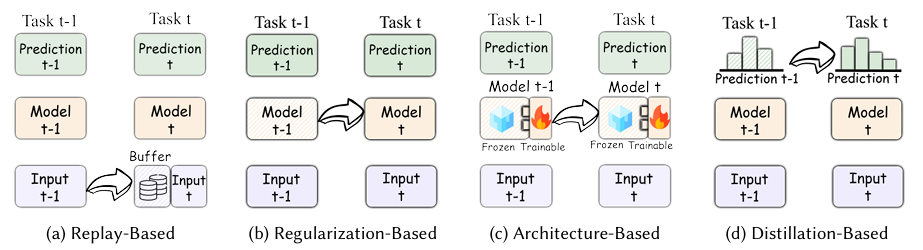
\includegraphics[scale=.45]{Images/Chapter2/llm_methods.png}
\caption[]{طبقه‌بندی روش‌های یادگیری پیوسته در مدل‌های بینایی بزرگ و بینایی-زبان  \protect\cite{llm_continual}}
\label{fig.21}
\end{figure}


\subsection{روش‌های مبتنی بر تنظیم}
در این روش، مدل از مکانیزم‌هایی مانند جریمه یا محدودسازی برای حفظ اطلاعات قبلی استفاده می‌کند. هدف این است که پارامترهایی که در یادگیری گذشته مهم بوده‌اند، هنگام آموزش جدید کمتر تغییر کنند. در این روش، در صورت حجم زیاد وظایف، اثربخشی کاهش می‌یابد
\cite{llm_continual}
.

\subsection{روش‌های مبتنی بر تقطیر دانش}
مدل دانش خود را از مدل‌های قبلی یا معلم یاد می‌گیرد و توجه به مواردی مانند حساسیت به دقت مدل معلم و انتخاب صحیح داده‌ها برای تقطیر حائز اهمیت است
\cite{llm_continual}.
لو و همکاران 
\cite{distillation}،
با هدف کاهش فراموشی در یادگیری افزایشی ویدیو، از روشی به نام تقطیر توجه \LTRfootnote{Attention distillation} استفاده کرده‌اند که در آن ویژگی‌های توجه از خروجی کدگشای ترنسفورمر \lr{CLIP}، به مدل جدید منتقل می‌شود. این رویکرد به مدل کمک می‌کند تا دانش مراحل قبلی را حفظ کرده و در عین حال بتواند دسته‌های جدید را بدون نیاز به آموزش کامل مجدد یاد بگیرد. 


\subsection{روش‌های مبتنی بر معماری}
در این رویکرد، معماری مدل برای جذب وظایف جدید، بدون تداخل با وظایف قبلی، تغییر می‌کند؛ مانند افزودن پیمانه
\LTRfootnote{Module}
 استفاده از تطبیق‌دهنده‌ها و .... 
 ژنگ و همکاران
\cite{llm_continual}،
با بررسی روش‌های مختلف ارائه‌شده در این رویکرد، طبقه‌بندی مطابق با 
\cref{fig.22}
ارائه داده اند که در ادامه به بررسی آن‌ها پرداخته‌ می‌شود
.
\begin{figure}
\centering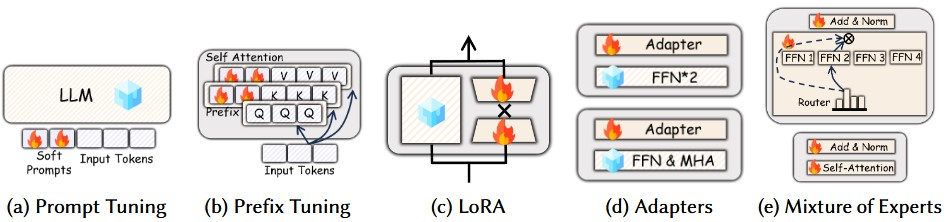
\includegraphics[scale=.75]{Images/Chapter2/llm_architec_methods.jpg}
\caption[]{ روش‌های یادگیری پیوسته مبتنی بر معماری در مدل‌های زبانی بزرگ و بینایی-زبان \protect\cite{llm_continual}}
\label{fig.22}
\end{figure}

\subsubsection{تنظیم پرامپت}
همانطور که در بخش یادگیری انتقالی مدل‌های بینایی-زبان ذکر شد، در روش تنظیم پرامپت، به‌جای بازآموزی کامل یا تغییر در پارامترهای اصلی مدل، مجموعه‌ای از بردارهای قابل‌ آموزش به‌عنوان پرامپت به ابتدای نشانه‌های ورودی
\LTRfootnote{Input tokens}
اضافه می‌شوند. این بردارها بدون دست‌کاری در ساختار درونی مدل، نقش راهنما را ایفا کرده و جهت‌گیری مدل در تفسیر داده‌های جدید را مشخص می‌سازند. در واقع، مدل با همان دانش قبلی خود به تحلیل ورودی می‌پردازد، اما به‌واسطه‌ی پرامپت‌های جدید، قادر به تطبیق با وظایف تازه می‌شود \cite{llm_continual}. این روش به‌دلیل مصرف کم منابع محاسباتی و عدم نیاز به تغییر در پارامترهای اصلی، به‌ویژه برای سناریوهایی با دسترسی محدود به مدل یا منابع، بسیار مناسب است و الگوی مورد استفاده در این روش، می‌تواند به خوبی برای مسائل یادگیری پیوسته نیز استفاده شود
\cite{llm_continual}.
\begin{figure}
	\centering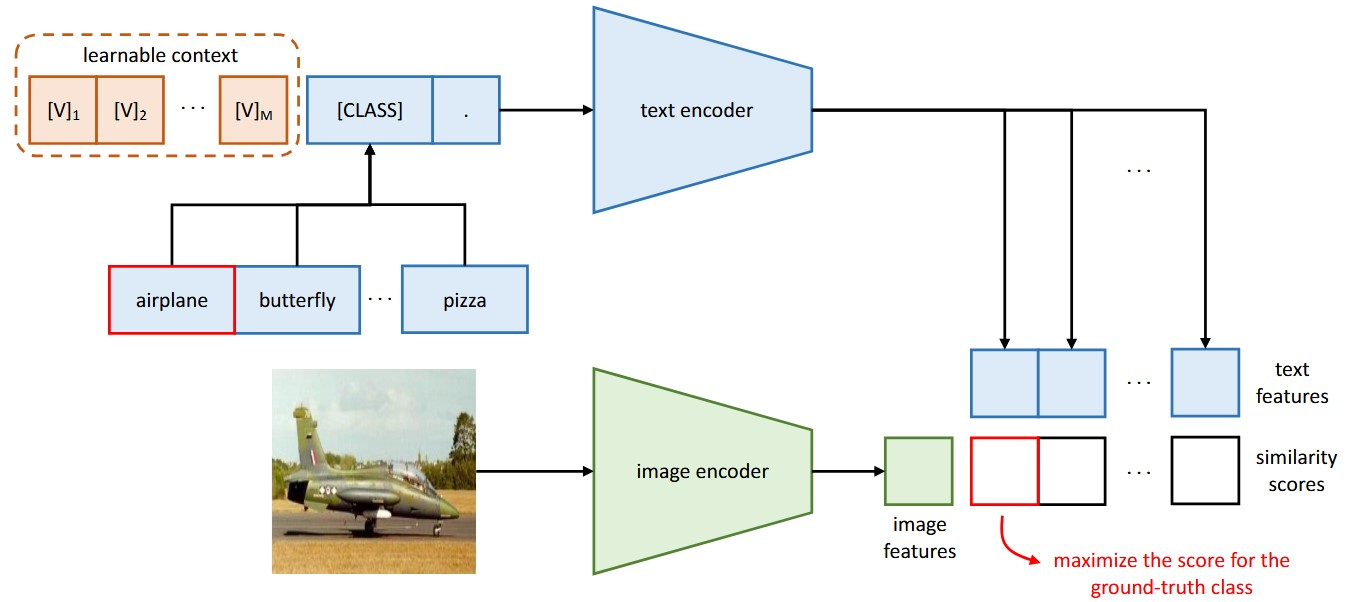
\includegraphics[scale=.55]{Images/Chapter2/CoOp.jpg}
	\caption[]{ نمایش روش 
		\lr{CoOp}
		\protect\cite{CoOp}}
	\label{fig.23}
\end{figure}
\begin{figure}
	\centering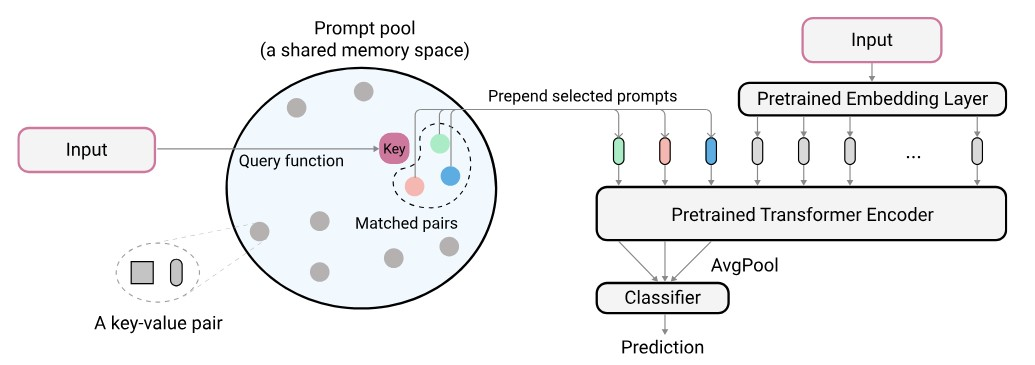
\includegraphics[scale=.65]{Images/Chapter2/l2p.jpg}
	\caption[]{ نمایش روش 
		\lr{L2P}
		در زمان آزمون
		\protect\cite{l2p}}
	\label{fig.24}
\end{figure}
ژو و همکاران 
\cite{CoOp}،
رویکردی به نام بهینه‌سازی بافت 
\LTRfootnote{Context Optimization (CoOp)}
(که در بخش قبل اشاره شد) ارائه کرده‌اند که به جای پرامپت‌های ثابت، از پرامپت به صورت بردارهای بافت یادگرفتنی
\LTRfootnote{Learnable context vectors}
که در کنار برچسب متنی داده‌ها قرار می‌گیرند، استفاده می‌کند. مطابق 
\cref{fig.23}،
تمام وزن‌های مدل 
\lr{CLIP}،
ثابت نگه داشته شده و تنها بردارهای پرامپت، قابل‌آموزش هستند. به دنبال توسعه ی روش های پرامپت گذاری، روش
\lr{L2P}
\LTRfootnote{Learning to Prompt for Continual Learning}
که توسط وانگ و همکاران
\cite{l2p}
ارائه شده است، یک چارچوب نوآورانه برای یادگیری پیوسته بدون نیاز به شناسایی وظیفه در زمان آزمون می‌باشد. همان‌طور که در 
\cref{fig.24}
مشاهده می‌شود، این روش به جای تغییر وزن‌های مدل پیش‌آموخته، از مجموعه‌ای از پرامپت‌های یادگرفتنی بهره می‌برد که در یک فضای حافظه اشتراکی به نام استخر پرامپت
\LTRfootnote{Prompt pool}
نگهداری می‌شوند. 
\lr{L2P}
از یک مکانیزم پرس‌وجوی مبتنی بر جفت‌های کلید-مقدار بهره می‌برد تا به‌صورت پویا و متناسب با ورودی، پرامپت‌های مرتبط را انتخاب کرده و به نشانه‌‌های ورودی مدل، اضافه کند. سپس این نشانه‌‌های توسعه‌یافته به مدل پیش‌آموخته تزریق شده و پیش‌بینی انجام می‌شود.
در این روش، پرامپت‌ها، دانش خاص هر وظیفه یا دانش مشترک بین وظایف را به‌صورت فشرده ذخیره می‌کنند و باعث کاهش چشمگیر فراموشی مخرب در یادگیری وظایف متوالی می‌شوند. ساختار طراحی‌شده در  
\lr{L2P}
همان‌طور که در 
\cref{fig.24}
نشان داده شده، از یک بخش انتخاب پرامپت، لایه‌های کدگذار پیش‌آموخته
\LTRfootnote{Pretrained encoder layers}،
و دسته‌بند نهایی تشکیل شده است. جهت بهبود و مقاوم‌سازی نسبت به فراموشی در انتخاب پرامپت روش‌های پیشین، مارتین و همکاران
\cite{starprompt}،
روش 
\lr{STAR-Prompt}
را معرفی کرده‌اند که از رویکردی دوسطحی برای تنظیم پرامپت، پیروی می‌کند. ابتدا از 
\lr{CLIP}،
برای تولید پرامپت‌های متنی و ساخت نمونه‌های‌ اولیه
\LTRfootnote{Prototypes}
پایدار دسته‌ها، استفاده می‌شود و سپس این نمونه‌های اولیه به‌عنوان کلید برای بازیابی پرامپت‌های تصویری در ترنسفورمر تصویر به‌کار می‌روند. هم‌چنین روش‌های
\lr{DualPrompt}
\cite{dual-prompt}
و 
\lr{H-prompts}
\cite{h-prompts}،
مانند مطالعات مذکور، در زمینه‌ی تولید پرامپت‌های مشترک و خاص وظایف ارائه شده‌اند. داهویین و همکاران
\cite{instance_prompt}،
از پرامپت اختصاصی برای هر نمونه به‌جای هر‌دسته، استفاده کرده‌اند. برخلاف روش‌های پرامپت‌گذاری قبلی، هنگ و همکاران
\cite{ovor}،
علاوه بر استفاده از یک پرامپت به‌جای چندپرامپت، از نمونه‌های پرت مصنوعی برای ایجاد مرز دسته‌بندی بهتر استفاده کرده‌اند. در مطالعات دیگری مانند روش یکپارچه‌سازی دانش بدون تداخل و آگاه از توزیع
\cite{diki}
\LTRfootnote{Distribution-aware Interference-free Knowledge Integration (DIKI)}،
به رفع چالش مداخله‌ی پرامپت در تصمیم‌گیری مکانیزم توجه پرداخته شده است. به دنبال پیشرفت‌های روش‌های پرامپت در حوزه‌ی تصویر، ویلا و همکاران
\cite{pivot}،
روشی به نام
\lr{PIVOT}
را معرفی کرده‌اند که با بهره‌گیری از دانش پیش‌آموخته مدل‌ تصویر-متن
\lr{CLIP}
و استفاده از پرامپت‌های مکانی
\LTRfootnote{Spatial prompts}
و زمانی، وابستگی‌های زمانی و مکانی ویدیوها را مدل کرده است. وانگ و همکاران \cite{clip-poolprompt} نیز با هدف ارتقای عملکرد مدل \lr{CLIP} در تشخیص حرکت‌های انسانی در ویدیوها، چارچوبی معرفی کرده‌اند که با استفاده از مدل‌سازی حرکتی و پرامپت‌های پویا، به شکلی مؤثر اطلاعات حرکتی را وارد فرآیند یادگیری می‌کند بدون اینکه به تغییر پارامترهای اصلی \lr{CLIP} نیاز باشد. در مواردی نیز مانند روش \lr{ViLT-CLIP} 
\cite{vilt-clip}،
از هر دو نوع پرامپت برای تصویر و متن برای درک ویژگی‌های ویدیویی استفاده شده‌است.

 
\subsubsection{تنظیم پیشوند}
 در روش تنظیم پیشوند \LTRfootnote{Prefix tuning}، مجموعه‌ای از پارامترهای قابل آموزش به عنوان پیشوند به ابتدای هر لایه‌ی ترنسفورمر افزوده می‌شود تا رفتار مدل را در انجام وظایف خاص تنظیم کند. این پیشوندها نقش تغییرات زمینه‌ای را ایفا کرده و برخلاف تنظیم پرامپت، چندین لایه از مدل را تحت تأثیر قرار می‌دهند \cite{llm_continual}. روی و همکاران \cite{prefix-tuning}، روشی معرفی کرده‌اند که با استفاده از پیشوندهای قابل یادگیری در هر لایه‌ی مدل، امکان یادگیری وظایف جدید را بدون فراموشی وظایف قبلی فراهم می‌کند. این پیشوندها با ترکیب کانولوشن و اطلاعات مشترک بین وظایف، باعث انتقال بهتر دانش و کاهش تعداد پارامترهای لازم در یادگیری پیوسته می‌شوند.
 
\subsubsection{سازگار‌سازی رتبه‌پایین}
 با وارد کردن ماتریس‌های رتبه‌پایین در لایه‌های معینی از مدل پیش‌آموخته و منجمد، روش سازگار‌سازی رتبه‌پایین \LTRfootnote{Low‑Rank Adaptation (LoRA)}، امکان تنظیم هدفمند بخش‌هایی از مدل را بدون بازآموزی کامل فراهم می‌سازد \cite{llm_continual}. مارتین و همکاران \cite{lora}، به نتیجه رسیدند که در زمینه‌ی یادگیری پیوسته، جایگزینی روش مذکور به‌جای تنظیم پرامپت، بدون افزایش چشمگیر در تعداد پارامترها، منجر به بهبود عملکرد مدل می‌گردد.
 
\subsubsection{وفق دهنده}
همانطور که در بخش یادگیری انتقالی مدل‌های بینایی-زبان ذکر شد، وفق دهنده‌ها شبکه‌های عصبی کوچک با ساختار فشرده‌ای هستند که بین لایه‌های مدل اصلی قرار می‌گیرند و به مدل امکان می‌دهند ویژگی‌های جدید را یاد بگیرد، بدون آن‌که نیازی به تغییر پارامترهای اصلیِ از پیش آموزش‌دیده باشد \cite{llm_continual}. به همین دلیل، می‌توان این روش را نیز در یادگیری پیوسته استفاده نمود. در برخی روش‌ها مانند 
\lr{DIA}
\cite{dia-adapter-2025}
و 
\lr{EASE}
\cite{ease-adapter-2024}،
از وفق دهنده‌های سبک‌وزن و اختصاصی برای هر وظیفه‌ی جدید استفاده می‌شود تا مدل بتواند بدون بازآموزی کامل یا ذخیره داده‌های قدیمی، دانش جدید را جذب کند. این دو روش، امکان به‌روزرسانی مدل را بدون آسیب به دانش قبلی فراهم کرده و تصمیم‌گیری ترکیبی میان دسته‌های قدیم و جدید را ممکن می‌سازند. دانگ و همکاران 
\cite{cada-adapter-2025}،
در مطالعه‌ای دیگر، روشی به نام \lr{C-ADA}، ارائه داده‌اند که با استفاده از وفق دهنده‌هایی با قابلیت گسترش پارامتری، یادگیری وظایف جدید را بدون نیاز به ذخیره داده‌های گذشته ممکن می‌سازد. این روش با حفظ پارامترهای قبلی و افزودن وزن‌های جدید، از تداخل دانش جلوگیری کرده و عملکرد و سرعت آموزش را به‌طور محسوسی بهبود می‌دهد. برای رفع چالش تداخل پارامترهای دسته‌های مشابه در یادگیری پیوسته، هانگ و همکاران 
\cite{rapf-adapter-2024}،
با استفاده از وفق دهنده‌های قابل تنظیم، ابتدا بازنمایی‌های متنی را متناسب با تأثیر دسته‌های جدید بر دسته‌های قدیمی اصلاح می‌کنند و سپس با یک راه‌برد تجزیه و ادغام پارامترها، فراموشی مدل در حین تنظیم وفق دهنده‌ها را کاهش می‌دهند. در حوزه‌ی ویدیو نیز، پن و همکاران 
\cite{st-adapter-2022}،
روشی به نام \lr{ST-Adapter} پیشنهاد داده‌اند که با افزودن قابلیت زمانی-مکانی به مدل‌ تصویری از پیش‌آموخته، آن را برای وظایف ویدیویی قابل استفاده کرده است. 
 
\subsubsection{مخلوط خبره‌ها}
 روش مخلوط خبره‌ها
\LTRfootnote{Mixture of Experts (MoE)}،
 با استفاده از یک مکانیزم دروازه‌ای، به‌صورت پویا تعدادی از شبکه‌های عصبی خبره را برای انجام هر وظیفه فعال می‌کند. این ساختار باعث می‌شود مدل بخش‌های مختلف خود را به وظایف متنوع اختصاص دهد و عملکرد بهتر و مقیاس‌پذیری بیشتری پیدا کند. ونگ و همکاران 
\cite{sema-2024}،
در این زمینه رویکردی را ارائه داده‌اند که مدل به‌صورت خودکار تصمیم می‌گیرد که بسته به تغییر داده یا وظیفه، از کدام وفق دهنده‌های موجود استفاده کند یا وفق دهنده‌ی جدیدی اضافه نماید، تا تعادلی میان حفظ دانش قبلی و یادگیری دانش جدید ایجاد شود. در ادامه نیز، یو و همکاران 
\cite{ddas-2024}،
با استفاده از همین روش و با گسترش تدریجی مدل \lr{CLIP} و استفاده از مسیرهای انتخابی میان وفق دهنده‌های خبره و مدل اصلی، قابلیت تشخیص یادگیری بدون نمونه حفظ شده و در عین حال بار محاسباتی به شکل چشم‌گیری کاهش می‌یابد.

 

 
 
 
 
 
 
 
 
 
 
 
 
 
 
 
 
 
 
 
 
 
 
 
 
 

\chapter{روش پیشنهادی}
%\thispagestyle{empty}

\section{مقدمه}

روش‌های موجود در زمینه یادگیری پیوسته برای داده‌های ویدیویی با وجود پیشرفت‌های اخیر، همچنان با مشکلات اساسی روبه‌رو هستند. برخی رویکردها به مدل‌های از پیش آموزش‌دیده متکی‌اند، اما برای انطباق با داده‌های ویدیویی نیاز به آموزش یا تنظیم مجدد کدگذارهای زمانی دارند، که فرآیندی زمان‌بر، پرهزینه و وابسته به منابع سخت‌افزاری سنگین است \cite{pivot}. هم‌چنین، روش‌های مختلف (تصویر یا ویدیو)، برای مقابله با فراموشی فاجعه‌بار به استفاده از بافرهای بازپخش یا ذخیره‌سازی داده‌های قبلی متکی هستند که نیازمند حافظه بالا و ناسازگار با محدودیت‌های حریم خصوصی است
\cite{pivot,9,memory-1}
. علاوه بر این، برخی از روش‌ها از ساختارهای وابسته به وظیفه
\LTRfootnote{Task specific}
استفاده می‌کنند که مدیریت و نگهداری آن‌ها در سناریوهای واقعی و وظایف متوالی دشوار بوده و باعث کاهش تعمیم‌پذیری می‌شود \cite{task-specific-1,task-specific-2}.

با توجه به این محدودیت‌ها، نیاز به رویکردهایی احساس می‌شود که بتوانند بدون وابستگی به ذخیره‌سازی وسیع داده‌های گذشته یا آموزش سنگین کدگذارها، عملکرد بهتری در داده‌های ویدیویی ارائه دهند و در عین حال ماهیت مستقل از وظیفه
\LTRfootnote{Task-agnostic}
 داشته باشند. هدف چنین رویکردهایی این است که از ظرفیت مدل‌های بزرگ و از پیش آموزش‌دیده استفاده کرده و با اضافه کردن لایه‌های سبک یا پرامپت‌های یادگیرنده، بدون تغییر مستقیم پارامتر‌های اصلی مدل، دانش قبلی را حفظ کنند و با داده‌های جدید تطبیق یابند.

در راستای رفع محدودیت‌های مذکور، در این فصل به ارائه روشی با عنوان
\lr{ProActionCLIP}\RTLfootnote{این نام مخفف \lr{Prompt Action recognition CLIP} 
	می‌باشد که به استفاده از روش‌ پرامپت‌گذاری برای تشخیص حرکت توسط مدل کلیپ، اشاره می‌کند.
}،
پرداخته‌ می‌شود که با ترکیب قابلیت‌های روش
\lr{Open-VCLIP}~\cite{open-vclip}
و ایده‌های روش
\lr{L2P}~\cite{l2p}، 
از پرامپت‌های سبک و پویا، برای انطباق با وظایف جدید، استفاده می‌کند. بنابراین در این روش، نیازی به طی کردن فرآیند آموزش کدگذارهای زمانی، که از نظر محاسباتی هزینه‌بر است، وجود ندارد.
روش \lr{ProActionCLIP}، با بهره‌گیری بهینه از دانش مدل‌های پیش‌آموزش‌دیده، کاهش فراموشی فاجعه‌بار و حفظ کارآیی در سناریوهای واقعی را هدف قرار داده است. این روش می‌تواند با بهره‌گیری بهینه از منابع محاسباتی و نیاز کمتر به سخت‌افزار، توانایی یادگیری پیوسته وظایف جدید را داشته باشد و بدون وابستگی به شناسه وظایف، عملکردی کارآمد و مقیاس‌پذیر ارائه دهد.

\section{روش \lr{ProActionCLIP}}
<<<<<<< HEAD
در این بخش، روش پیشنهادی برای یادگیری پیوسته‌ی تشخیص حرکت انسان معرفی می‌شود که بر پایه‌ی ترکیب دو رویکرد \lr{Open-VCLIP} و \lr{L2P}، بنا شده است. ایده‌ی اصلی این روش آن است که از قابلیت‌های \lr{Open-VCLIP} برای استخراج ویژگی‌های چندماهیتی (تصویر-متن) بهره گرفته و در عین حال از سازوکار پرامپت‌های یادگیرنده در \lr{L2P} استفاده شود تا مدل بتواند بدون نیاز به تغییر مستقیم پارامتر‌های کدگذار اصلی، خود را با وظایف متوالی تطبیق دهد. این ترکیب باعث می‌شود که مشکل فراموشی فاجعه‌بار کاهش یافته، حافظه‌ی مورد نیاز برای ذخیره‌سازی نمونه‌ها به حداقل برسد و مدل به صورت مستقل از وظیفه، وظایف جدید را یاد بگیرد. به عبارت دیگر، با این رویکرد سعی شده است مزیت‌های هر دو روش با هم ترکیب شود که عبارت‌اند از: قدرت تعمیم‌دهی و دانش وسیع \lr{Open-VCLIP} و انعطاف‌پذیری \lr{L2P} در مدیریت وظایف پیوسته. مدل \lr{ProActionCLIP}، شامل دو مرحله‌‌ی آموزش  و آزمون می‌باشد که پس از معرفی مدل‌های پایه‌‌ی بکار برده شده در مدل، به توضیح آن‌ها پرداخته می‌شود.

\section{مدل \lr{Open-VCLIP}}
مدل‌های بینایی-زبان مانند \lr{CLIP}، به دلیل توانایی یادگیری بازنمایی‌های مشترک تصویر و متن، عملکرد قابل توجهی در وظایف بینایی و زبانی داشته‌اند. با این حال، این مدل‌ها در حالت پایه برای داده‌های ایستا (تصاویر) طراحی شده‌اند. \lr{Open-VCLIP} با گسترش معماری \lr{CLIP} و افزودن قابلیت درک اطلاعات زمانی، این محدودیت را برطرف می‌کند و روشی کارآمد برای تحلیل ویدیو ارائه می‌دهد. هم‌چنین برای جلوگیری از فراموشی اطلاعات مدل \lr{CLIP} پس از یادگیری داده‌های ویدیویی، از دو تکنیک \LTRfootnote{Technique} به نام‌های منظم‌سازی وزن‌های میان‌یابی \LTRfootnote{Interpolation Weight Regularization (IWR)} و میانگین تصادفی وزن‌ها \LTRfootnote{Stochastic Weight Averaging (SWA)} استفاده می‌کند. تکنیک اول با بکارگیری روش ترکیب مدل قدیمی و جدید و تغییراتی در آن، از فراموشی دانش قبلی جلوگیری کرده و هم‌زمان باعث یادگیری دانش جدید می‌شود. در تکنیک دوم، با میانگین‌گیری از وزن‌های مدل در نقاط مختلف، باعث بهبود وزن‌های نهایی از لحاظ تعمیم‌پذیری می‌شوند. هر یک از این تکنیک‌ها در ادامه به تفصیل، شرح داده خواهد شد. 
=======
روش
\lr{ProActionCLIP}،
که برای یادگیری پیوسته‌ی تشخیص حرکت انسان معرفی شده، بر پایه‌ی ترکیب دو رویکرد
\lr{Open-VCLIP}
و
\lr{L2P}،
بنا شده است. ایده‌ی اصلی این روش آن است که از قابلیت‌های \lr{Open-VCLIP} برای استخراج ویژگی‌های چندماهیتی (تصویر-متن) بهره گرفته و در عین حال از سازوکار پرامپت‌های یادگیرنده در \lr{L2P} استفاده می‌کند. به‌این‌ترتیب مدل می‌تواند بدون نیاز به تغییر مستقیم پارامتر‌های کدگذار اصلی، خود را با وظایف متوالی تطبیق دهد. این ترکیب باعث می‌شود که مشکل فراموشی فاجعه‌بار کاهش یافته، حافظه‌ی مورد نیاز برای ذخیره‌سازی نمونه‌ها به حداقل برسد و مدل به صورت مستقل از وظیفه، وظایف جدید را پردازش کند. به عبارت دیگر، با این رویکرد سعی شده است مزیت‌های هر دو روش با هم ترکیب شود که عبارت‌اند از: قدرت تعمیم‌دهی و دانش وسیع \lr{Open-VCLIP} و انعطاف‌پذیری \lr{L2P} در مدیریت وظایف پیوسته. مدل \lr{ProActionCLIP}، شامل دو مرحله‌‌ی آموزش  و آزمون می‌باشد که پس از معرفی مدل‌های پایه‌‌ی بکار برده شده در
\lr{ProActionCLIP}،
به توضیح آن‌ها پرداخته می‌شود.

\section{مدل \lr{Open-VCLIP}}
مدل‌های بینایی-زبان مانند \lr{CLIP}، به دلیل توانایی یادگیری نمایش‌های مشترک تصویر و متن، عملکرد قابل توجهی در وظایف بینایی و زبانی داشته‌اند. با این حال، این مدل‌ها در حالت پایه برای داده‌های ایستا (تصاویر) طراحی شده‌اند. \lr{Open-VCLIP} با گسترش معماری \lr{CLIP} و افزودن قابلیت درک اطلاعات زمانی، این محدودیت را برطرف می‌کند و روشی کارآمد برای تحلیل ویدیو ارائه می‌دهد. 
مدل 
\lr{Open-VCLIP}
به ارائه دو تکنیک می‌پردازد که چالش فراموشی اطلاعات در مدل
\lr{CLIP}،
پس از یادگیری داده‌های ویدیویی، را تا حد خوبی برطرف می‌کند.

>>>>>>> 3dfeaaefeb6cdef3ce3e29e5b3b36b35ee62708a
\subsection{تبدیل \lr{CLIP} مبتنی بر تصویر به \lr{CLIP} مبتنی بر ویدیو}
در این بخش، ورودی ویدیویی به دنباله‌ای از قاب‌‌ها تبدیل می‌شود و هر قاب توسط کدگذار تصویری \lr{CLIP} به یک بردار ویژگی تبدیل می‌گردد. سپس این ویژگی‌ها در قالب دنباله‌ای زمانی قرار گرفته و با سازوکار توجه ترکیب می‌شوند. در سازوکار توجه فرمول محاسبه‌ی خروجی مطابق \eqref{eq:attention_basic} می‌باشد.
\begin{equation}\label{eq:attention_basic}
	y_{s,t} = \mathrm{Softmax}\left( \frac{q_{s,t} K_{t}^{\mathrm{T}}}{\sqrt{d}} \right) V_{t},
\end{equation}
در این رابطه، $q_{s,t}$ بردار پرسمان \LTRfootnote{Query} برای یک وصله
	\LTRfootnote{Patch}
	 از تصویر، $K_t$ ماتریس کلید و $V_t$ ماتریس مقدار برای قاب یا تصویر $t$ هستند که از طریق سازوکار توجه ترکیب می‌شوند. در این حالت، ارتباط یک وصله از تصویر با خودش و بقیه‌ی وصله‌های تصویر مشخص می‌شود. برای سازگار کردن مدل برای ویدیو در مدل \lr{Open-VCLIP}، بردار پرسمان وصله‌ی قاب فعلی را در ماتریس کلید قاب فعلی، بعدی و قبلی ضرب می‌کند و پس از اجرای تابع \lr{softmax} نیز در ماتریس مقدار قاب فعلی، بعدی و قبلی ضرب می‌کند و سازوکار توجه را مانند \eqref{eq:attention_extended}، محاسبه می‌کند. در این صورت نه تنها ارتباط وصله‌ی قاب فعلی با قاب خودش، بلکه با قاب قبلی و بعدی خود نیز در نظر گرفته می‌شود (مطابق با \cref{fig.31}). این راهکار به ظاهر ساده، توانست تحول خوبی در زمینه‌ی سازگاری مدل \lr{CLIP} با داده‌ی ویدیویی ایجاد کند \cite{open-vclip}.
\begin{equation}\label{eq:attention_extended}
	y_{s,t} = \mathrm{Softmax}\left( 
	\frac{q_{s,t} \left[ K_{(t-1)\sim(t+1)} \right]^{\mathrm{T}}}{\sqrt{d}} 
	\right) 
	\left[ V_{(t-1)\sim(t+1)} \right],
\end{equation}

‌\begin{figure}
	\centering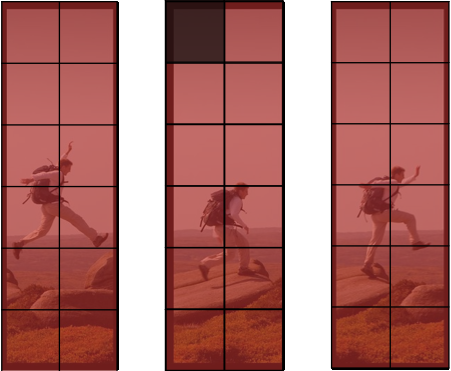
\includegraphics[scale=.50]{Images/Chapter3/openvclip_attention.png}
	\caption[]{ وصله‌های درنظر گرفته شده برای هر وصله از قاب در سازوکار تغییر یافته‌ی توجه}
	\label{fig.31}
\end{figure}

\subsection{منظم‌سازی وزن‌های میان‌یابی}
همانطور که ذکر شد، برای جلوگیری از فراموشی دانش پیش‌آموزش و در عین حال سازگار کردن مدل با داده‌های جدید، منظم‌سازی وزن‌های میان‌یابی معرفی شده است. در این روش، وزن‌های مدل به‌صورت ترکیبی از پارامتر‌های اولیه (پیش‌آموزش) و پارامتر‌های به‌روزرسانی‌شده در وظیفه جدید، تنظیم می‌شوند. این میان‌یابی به مدل کمک می‌کند تا در حین یادگیری، تعادلی میان دانش قدیمی و اطلاعات تازه برقرار کرده و از بیش‌برازش
 \LTRfootnote{Overfitting}
  جلوگیری کند. روش به‌کار رفته، تعمیم ایده‌ی گابریل و همکاران
  \cite{patchingmodels}،
 که مطابق با \eqref{eq:patching_model_base} است، می‌باشد.
\begin{equation}\label{eq:patching_model_base}
\theta = \lambda \theta_A + (1 - \lambda) \theta_B
\end{equation}

در این رابطه، $\theta$ از ترکیب خطی وزن‌های مدل پایه $\theta_A$ و مدل به‌روزرسانی‌شده $\theta_B$ با ضریب $\lambda$ تشکیل می‌شود تا صحت مدل در وظایف جدید افزایش یابد، بدون آنکه عملکرد آن در سایر وظایف که از پیش بهینه بوده‌اند، کاهش پیدا کند. با توجه به این که $\lambda$ یک ابرپارامتر \LTRfootnote{Hyper parameter} است، مقدار انتخابی آن، می‌تواند باعث بیش‌برازش یا زیربرازش روی داده‌های قبلی و جدید شود. پس به‌جای بهینه‌سازی مدل برای یک مقدار ثابت از $\lambda$، راه حلی باید ارائه شود که عملکرد مدل ترکیبی را در برابر بازه‌ای از مقادیر $\lambda$ بهینه کند. بنابراین، مطابق با \eqref{eq:patching_model_new}، وزن‌های جدید را در آموزش به سمتی می‌برد که هم زیان مدل جدید و هم زیان مدل ترکیبی با ضریب $\alpha$ روی داده‌های جدید حداقل شود. در این حالت، ترکیب‌های مختلف مدل قبلی و جدید در مراحل مختلف آموزش در نظر گرفته می‌شود که در واقع، عملکرد بهتری در تحلیل داده‌های نادیده خواهد داشت. در انتها مطابق با \eqref{eq:patching_model_base}، مدل جدید و قدیم ترکیب خواهند شد. با این تفاوت که وزن‌های مدل جدید، در طول آموزش با در نظر گرفتن عدم فراموشی مدل قبلی، یاد گرفته شده‌اند.
\begin{equation}\label{eq:patching_model_new}
	\arg \min_{\theta_B} \mathcal{L} =
	L(\theta_B; D_B) + \beta L\big(\alpha \theta_A + (1 - \alpha)\theta_B; D_B\big)
\end{equation}
پارامتر \( \alpha \) از یک توزیع یکنواخت در بازه \( (0, \lambda) \) نمونه‌برداری می‌شود و ضریب \( \beta \) به‌عنوان یک پارامتر تنظیم‌کننده برای کنترل میزان تاثیر عبارت میان‌یابی تعریف شده است. همچنین مقدار \( \beta \) به‌صورت \( \beta = C \frac{1}{1 - \alpha} \) محاسبه می‌شود که در آن \( C \) یک مقدار ثابت برای کنترل بزرگی \(\beta\) است. 

\subsection{میانگین‌گیری تصادفی وزن‌ها}
هم‌چنین به‌منظور تثبیت بیشتر مدل و بهبود قابلیت تعمیم آن، روش میانگین‌گیری تصادفی وزن‌ها\LTRfootnote{Stochastic Weight Averaging (SWA)} به کار گرفته شده است. در این مرحله، پارامتر‌های مدل جدید در طول چند مرحله از آموزش، ذخیره شده و میانگین آن‌ها به عنوان پارامتر نهایی انتخاب می‌شود. این رویکرد باعث کاهش نوسانات وزن‌ها و دستیابی به عملکرد پایدارتر در داده‌های آزمایشی می‌گردد. در نهایت، فرمول نهایی مدل مطابق با \eqref{eq:patching_model_final} خواهد بود.

\begin{equation}\label{eq:patching_model_final}
	\sum_{i}^{N} \frac{\lambda \theta_{A} + (1 - \lambda) \theta_{i}}{N}
	= \lambda \theta_{A} + (1 - \lambda)
	\left( \frac{1}{N} \sum_{i}^{N} \theta_{i} \right)
\end{equation}
بنابراین، مدل نهایی، تنظیم دقیق مدل \lr{CLIP} با تغییر سازوکار توجه بوده و برای جلوگیری از فراموشی مدل قبلی و حفظ قابلیت یادگیری بدون نمونه، دو تکنیک مناسب بکار گرفته شده است. 
\section{مدل \lr{L2P}}
روش ارائه‌شده در این مقاله، با هدف بهبود یادگیری پیوسته، از سازوکاری مبتنی بر «استخر پرامپت‌» استفاده می‌کند. در این رویکرد، به‌جای تغییر پارامتر‌های اصلی مدل، مجموعه‌ای از پرامپت‌های قابل‌آموزش طراحی می‌شود که مدل با استفاده از آن‌ها قادر به استخراج اطلاعات مهم از داده‌های ورودی است. در هر مرحله یادگیری، پرامپت‌های مناسب بر اساس شباهت با داده‌های جدید انتخاب می‌شوند و این امر باعث می‌شود مدل بتواند دانش جدید را یاد بگیرد، بدون آنکه دانش قبلی را فراموش کند. این روش با بهره‌گیری از معماری ترنسفورمر، توانسته است تعادل موثری میان حفظ دانش گذشته و یادگیری وظایف جدید برقرار کند. همانطور که در \cref{fig.32} قابل مشاهده است، این مدل دارای دو بخش انتخاب پرامپت‌ها و یادگیری و به‌روزرسانی پرامپت‌ها است که هر یک در ادامه توضیح داده‌ می‌شود.
‌\begin{figure}
	\centering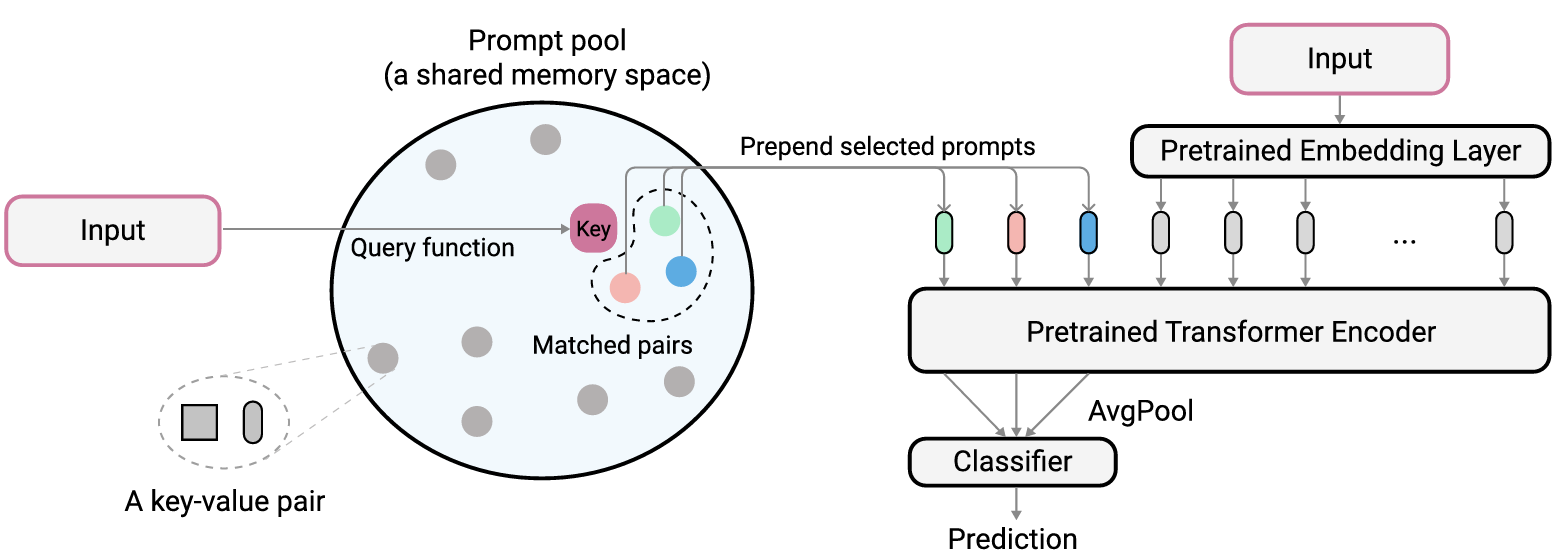
\includegraphics[scale=.38]{Images/Chapter3/l2p.png}
	\caption[]{ طرح کلی مدل \lr{L2P} \cite{l2p}}
	\label{fig.32}
\end{figure}

\subsection{انتخاب پرامپت}
در بخش انتخاب پرامپت\LTRfootnote{Prompt selection}، از استخر پرامپت تعدادی پرامپت متناسب با ورودی تصویری انتخاب می‌شود. استخر پرامپت شامل تعدادی پرامپت به تعداد $M$ بوده که به صورت \(\mathbf{P} = \{ P_{1}, P_{2}, \cdots, P_{M} \}\) نمایش داده‌ می‌شوند. هر \( P_j \in \mathbb{R}^{L_p \times D} \) یک پرامپت منفرد با طول نشانه‌ی \( L_p \) و اندازه تعبیه‌ی $D$ \LTRfootnote{Embedding size} مشابه تعبیه‌ی ورودی است. هم‌چنین هر پرامپت، دارای یک کلید است و فرآیند انتخاب بر اساس شباهت این کلیدها با بردار ویژگی مرتبط با کلاس ورودی انجام می‌گیرد. بردار ویژگی موردنظر از طریق استخراج‌کننده‌ی ویژگی، به‌دست می‌آید و سپس با کلیدهای موجود در استخر مقایسه می‌شود. در نهایت، تعدادی از پرامپت‌های کلیدهایی که بیشترین شباهت را با بردار ویژگی دارند انتخاب می‌شوند (مطابق با \cref{fig.32}). مجموعه‌ای از کلیدها به‌صورت 
\(\mathbf{K} = \{k_{j}\}_{i=1}^{M}\) 
نمایش داده می‌شود که هر \(k_i \in \mathbb{R}^{D_k}\) است. استخراج‌کننده‌ی ویژگی به صورت  \( q : \mathbb{R}^{H \times W \times C} \to \mathbb{R}^{D_k} \) معرفی می‌شود که بردار ویژگی \(x\) را به همان بعد کلیدها نگاشت می‌کند. در واقع از مدل ازپیش‌آموزش‌دیده به‌عنوان استخراج‌کننده ویژگی منجمد \LTRfootnote{Frozen} استفاده می‌شود:
\( q(x) = f(x)[0,:] \)
(که در آن از بردار ویژگی متناظر با کلاس استفاده می‌شود). 
تابع \(\gamma : \mathbb{R}^{D_k} \times \mathbb{R}^{D_k} \to \mathbb{R}\) به‌عنوان معیاری برای سنجش میزان تطابق بین بردار ویژگی ورودی و کلید پرامپت تعریف می‌شود (مانند فاصله کسینوسی). برای یک ورودی \(x\)، از تابع \(q(x)\) استفاده می‌کنیم تا بهترین \(N\) کلید انتخاب شوند. در نهایت، انتخاب کلید طبق \eqref{eq:prompt_selection} صورت می‌گیرد.
\begin{equation}\label{eq:prompt_selection}
	\mathbf{K}_x = 
	\underset{\{s_i\}_{i=1}^{N} \subseteq [1, M]}{\arg\min} 
	\sum_{i=1}^{N} \gamma \big( q(x), \mathbf{k}_{s_i} \big),
\end{equation}
\(\{s_i\}_{i=1}^{N}\) به‌عنوان یک زیرمجموعه از \(N\) کلید از بازه \([1, M]\) در نظر گرفته می‌شود
و \( \mathbf{K}_x \) نشان‌دهنده یک زیرمجموعه از بهترین \( N \) کلید انتخاب‌شده از \( \mathbf{K} \) به‌طور خاص برای نمونه \( x \) است.

علاوه بر این، به روش انتخاب پرامپت، قابلیت اضافه‌ای نیز اضافه شده است به این صورت که برای پرامپت‌های قبلا به‌روزرسانی شده، جریمه در نظر گرفته است تا متناسب با تعداد تکرارشان در وظایف قبلی، جریمه‌ی بیشتری برای انتخاب بگیرند. در این حالت، پرامپت‌های با تکرار کم نیز شانس انتخاب شدن پیدا می‌کنند و پرامپت‌ها با تکرار بیشتر، کمتر تغییر می‌کنند و تداخل کمتر می‌شود.
\subsection{یادگیری پرامپت}
در بخش یادگیری پرامپت، پرامپت‌های انتخاب‌شده به‌همراه داده‌ی ورودی به مدل تغذیه شده و پس از عبور از لایه‌های ترنسفورمر، بخش خروجی مربوط به پرامپت‌ها، استخراج شده و با میانگین‌گیری، به دسته‌بند \LTRfootnote{Classifier} منتقل می‌شود. سپس با انجام عملیات پس‌انتشار \LTRfootnote{Backpropagation}، وزن‌های پرامپت‌ها و کلیدهای متناظر آن‌ها به‌روزرسانی می‌شوند. این فرآیند باعث می‌شود مدل ضمن یادگیری وظایف جدید، قابلیت تعمیم خود را افزایش داده و دانش قبلی را حفظ کند (مطابق با \cref{fig.32}). تابع زیان در این مدل مطابق با \eqref{eq:l2p_loss}، به صورت ترکیبی معرفی می‌شود به این صورت که بخش اول شامل زیان بین برچسب تصویر و پیش‌بینی دسته‌بند از ورودی دارای پرامپت و بخش دوم شامل تفاوت بین کلیدهای انتخاب شده و ویژگی استخراجی از ورودی می‌باشد. به عبارتی تلاش بر این است که علاوه بر تقویت پرامپت‌ها، کلیدهای مرتبط نیز، به ویژگی ورودی متناظرشان نزدیک‌‌‌تر شوند. 
\begin{equation}\label{eq:l2p_loss}
	\min_{\mathbf{P}, \mathbf{K}, \phi} 
	\mathcal{L}\big( g_{\phi}( f_r^{\mathrm{avg}} (x_p) ), y \big) 
	+ \lambda \sum_{\mathbf{K}_x} \gamma \big( q(x), \mathbf{k}_{s_i} \big)
\end{equation}
همانطور که دیده می‌شود، بخش اول شامل تابع زیان (کراس انتروپی) بین خروجی دسته‌بند \(g_{\phi}\) و برچسب واقعی \(y\) محاسبه می‌شود. تابع \( f_r^{\mathrm{avg}} = \mathrm{AvgPool}(f_r(x_p)[0 : N L_p, :]) \)، به این معناست که بردارهای پنهان خروجی متناظر با مکان‌های \( N \cdot L_p \) پرامپت‌ها، پیش از ورود به لایه‌ی دسته‌بند، به‌صورت میانگین‌گیری شده ترکیب می‌شوند. 
در عبارت \( f_r(x_p) \)، تابع \( f_r \) نشان‌دهنده بخش باقی‌مانده از مدل ازپیش‌آموزش‌دیده است که پس از الحاق پرامپت‌ها به ورودی، عملیات پردازش ویژگی را انجام می‌دهد. 
بردار \( x_p \) نیز از اتصال پرامپت‌ها به بردار تعبیه‌شده ورودی حاصل می‌شود. در بخش دوم، پارامتر \(\lambda\) وزن اهمیت عبارت تنظیم‌کننده را مشخص می‌کند. فاصله بین بردار \(q(x)\) و کلیدهای انتخاب‌شده \(\mathbf{k}_{s_i}\) را کاهش می‌دهد. مجموعه \(\mathbf{K}_x\) نیز نشان‌دهنده کلیدهای انتخاب‌شده برای ورودی \(x\) است که طبق معادله \eqref{eq:prompt_selection} به دست می‌آیند.

در ادامه به توضیح مدل پیشنهادی و اجزای آن پرداخته می‌شود. 
\section{مرحله‌ی آموزش \lr{ProActionCLIP}}
همانطور که پیش‌تر اشاره شد، در مرحله‌ی آموزش، تمرکز بر یادگیری پرامپت‌های مناسب برای دسته‌های مختلفی است که به صورت پیوسته به مدل اضافه می‌شوند. طرح کلی مدل در مرحله‌ی آموزش در \cref{fig.33}، نشان داده شده است که الگو گرفته از مدل \lr{CLIP} می‌باشد. این مدل شامل یک کدگذار ویدیو (قابل به‌روزرسانی) و کدگذار متن منجمد (غیر قابل به‌روزرسانی) از مدل \lr{Open-VCLIP} است به این صورت که بردار ویژگی ویدیوی استخراج شده از کدگذار ویدیو و بردارهای ویژگی برچسب‌های موجود استخراج شده از کدگذار متن، طبق روش تقابلی مقایسه شده و طبق نزدیک شدن موارد متناظر و دور شدن موارد نامتناظر، وزن‌های پرامپت‌ها تغییر داده می‌شوند. دو بخش اصلی مدل به نام کدگذار ویدیو و یادگیری پرامپت در ادامه توضیح داده خواهند شد. 
‌\begin{figure}
	\centering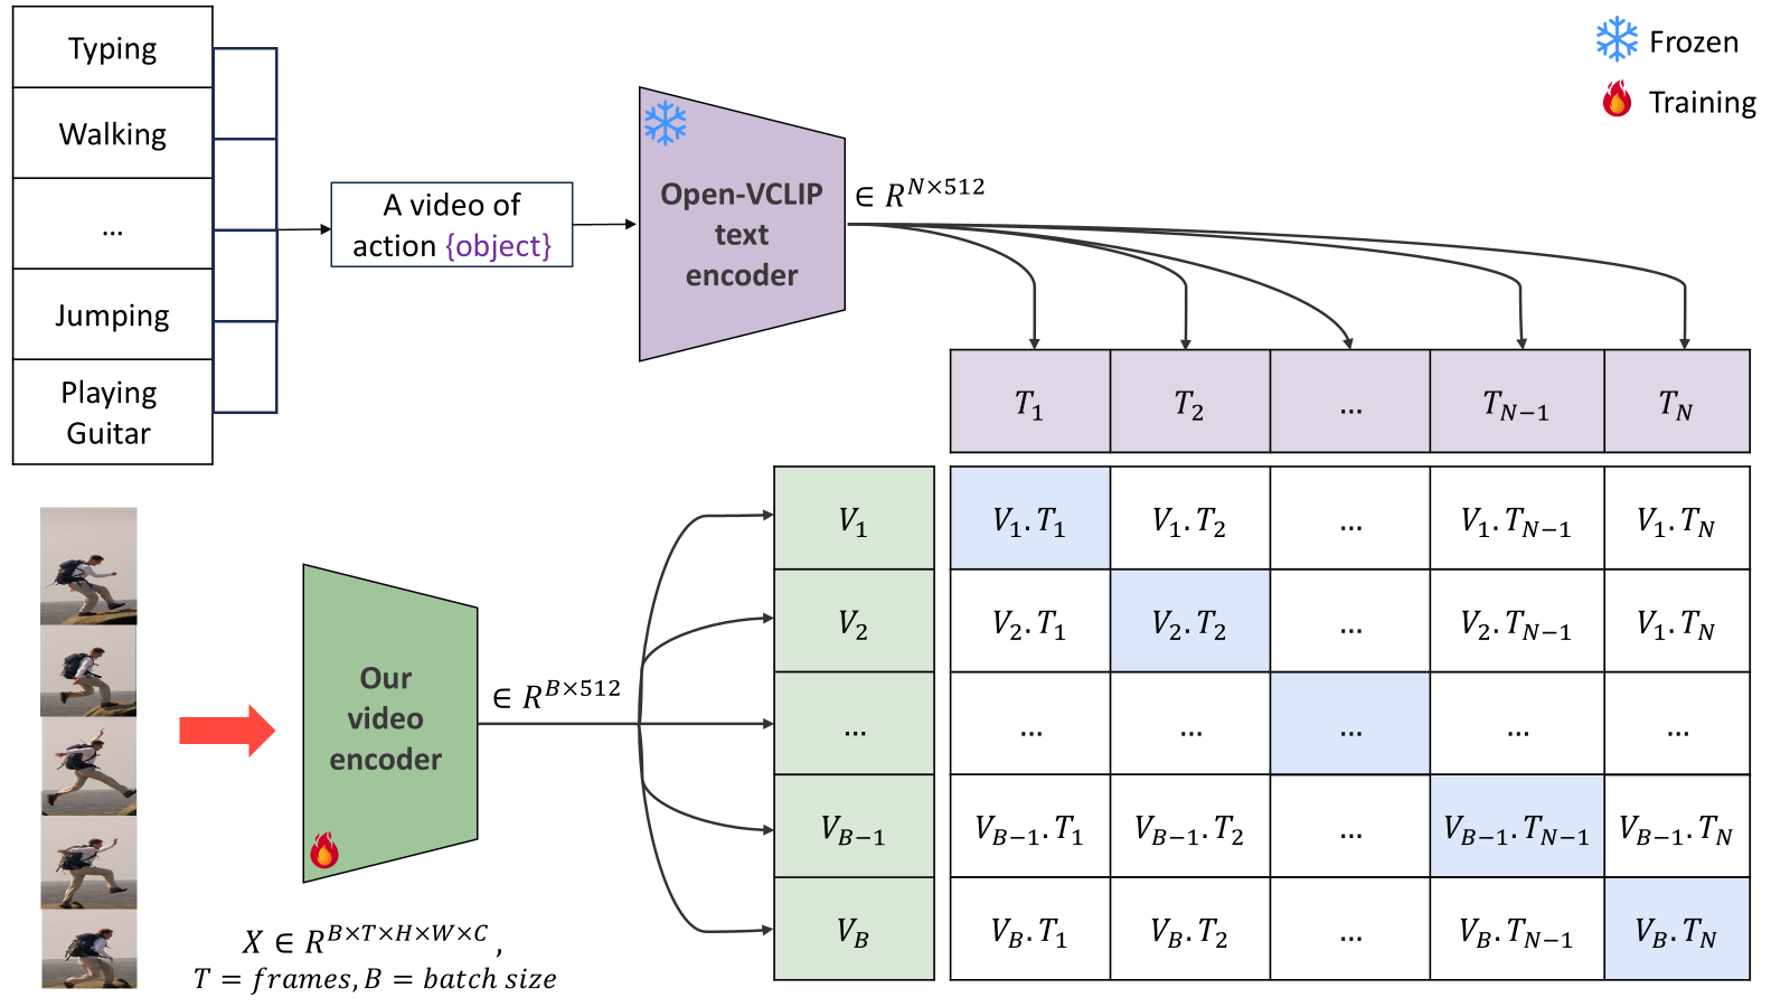
\includegraphics[scale=.50]{Images/Chapter3/train_phase.png}
	\caption[]{طرح کلی مرحله‌ی آموزش مدل \lr{ProActionCLIP}}
	\label{fig.33}
\end{figure}
\subsection{کدگذار ویدیو}
این بخش، از ترکیب \lr{L2P} و \lr{Open-VCLIP} تشکیل شده است. به طور کلی مطابق \cref{fig.34}، ویدیو به عنوان ورودی، وارد کدگذار \lr{Open-VCLIP} و لایه‌ی کانولوشنی دو‌بعدی می‌شود. ویژگی کلاس \LTRfootnote{Class feature (CLS)} از خروجی کدگذار \lr{Open-VCLIP} با 512 بعد، با کلیدهای داخل استخر پرامپت مقایسه می‌شود. به تعداد $N$ پرامپت از مشابه‌ترین کلیدها انتخاب می‌شوند. از طرف دیگر ویدیو از لایه‌ی کانولوشنی عبور کرده و پرامپت‌ها به هر قاب، به صورت جداگانه متصل می‌شوند. سپس به کدگذار ترنسفورمر معرفی شده در \lr{Open-VCLIP}، وارد شده و به ازای هر قاب، یک ویژگی کلاس بدست می‌آید که میانگین آن‌ها محاسبه و به عنوان خروجی نهایی این بخش، ارائه می‌گردد. در مدل پیشنهادی، صرفا پرامپت‌ها و کلیدهای متناظر آن‌ها، قابل یادگیری هستند و بقیه‌ی اجزا به صورت منجمد استفاده می‌شوند. در این بخش از تحقیق، آزمایش‌های مختلفی اجرا شد که بر اساس نوع انتخاب پرامپت و شرایط استخر پرامپت می‌توان به دسته‌‌های زیر تقسیم نمود:
\begin{itemize}
\item \textbf{مقداردهی اولیه‌ی کلید پرامپت:}
از آن جایی که ابتدای آموزش، مقادیر اولیه به صورت تصادفی هستند، در این آزمایش، مقادیر کلیدها، معادل ویژگی‌های برچسب دسته‌های استخراج شده از کدگذار متن قرار داده شد. در این صورت، مقایسه‌ی ویژگی ویدیو و کلیدها به صورت بهینه‌تر و دقیق‌تری صورت می‌گیرد. 
\item \textbf{وزن‌دهی به کلید پرامپت‌های از قبل انتخاب شده:}
مطابق با روش اضافه‌ای که برای انتخاب پرامپت در \lr{L2P} مطرح شد، تعداد تکرار پرامپت‌ها در هر وظیفه محاسبه می‌شود. در وظیفه‌ی بعدی، هرچه تکرار پرامپت بیشتر بوده باشد، تاثیرش در انتخاب کمتر می‌شود. 
\item \textbf{منجمد کردن پرامپت‌های قبلی:}
یکی از راه‌های استفاده از وزن‌های قبلی، این است که به صورت منجمد استفاده شوند و به‌روزرسانی نشوند. این روش کمک می‌کند اطلاعات اختصاصی هر وظیفه از بین نرود و اگر داده‌ی جدید اشتراکی با قبلی‌ها داشته باشد، پرامپت آن‌ها را انتخاب خواهد کرد.
\item \textbf{پویا بودن تعداد پرامپت‌های استخر پرامپت:}
در فرض اولیه، در استخر پرامپت تعدادی ثابت پرامپت وجود داشت اما برای بهینه‌بودن مدل برای دسته‌های بیشتر و موجود بودن پرامپت کافی در هر وظیفه، در این قسمت پرامپت‌ها در ابتدای هر وظیفه افزایش میابد. 

ترکیب برخی از این روش‌ها نیز آزمایش شده است مانند استفاده از استخر پویا و مقداردهی اولیه کلیدها.  
\end{itemize}
\begin{figure}
	\centering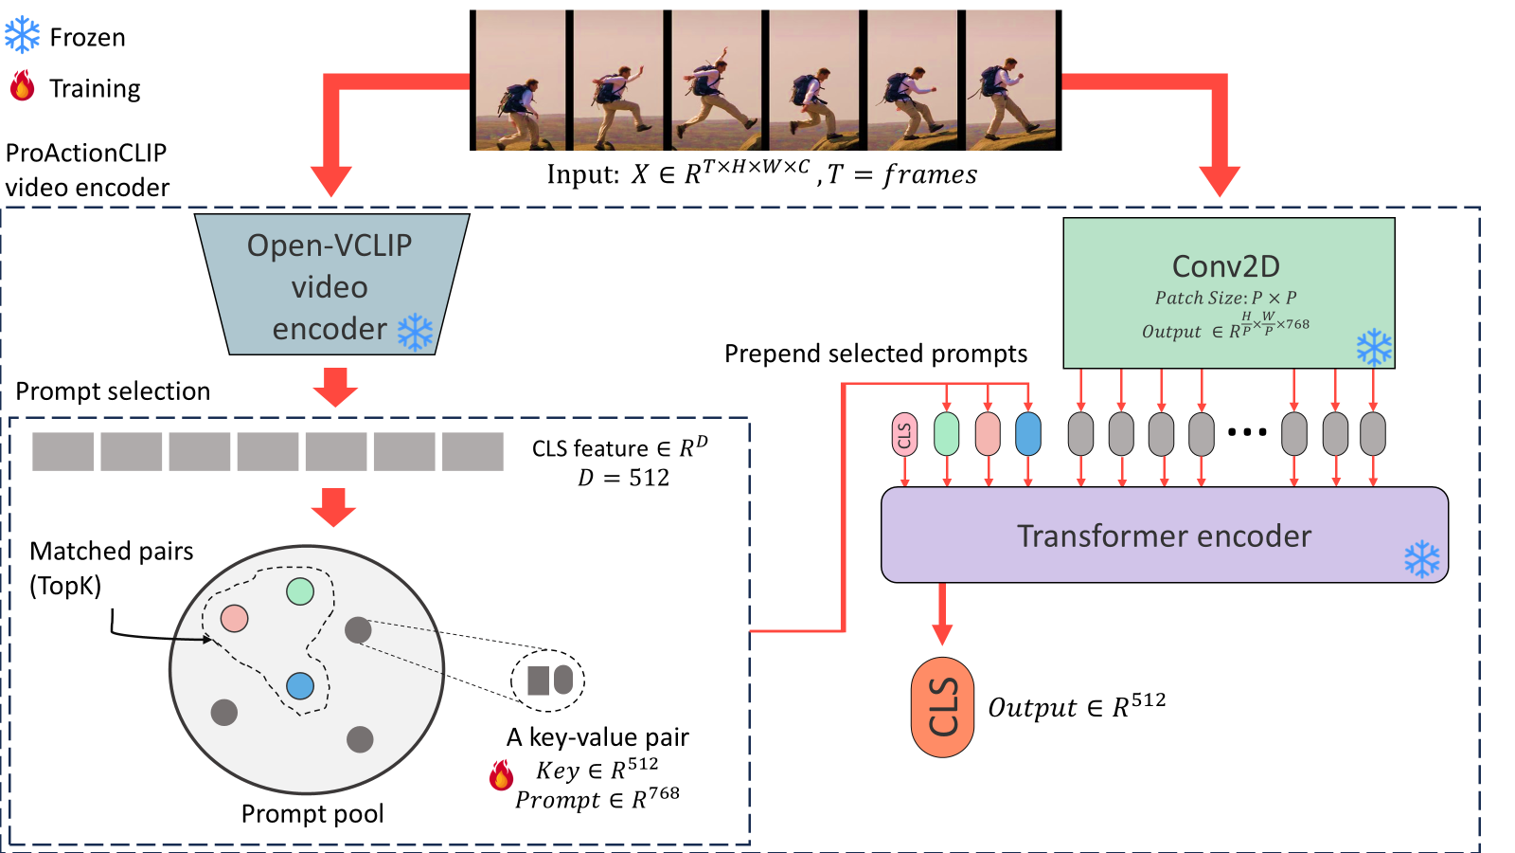
\includegraphics[scale=.65]{Images/Chapter3/video_encoder.png}
	\caption[]{سازوکار بخش کدگذار ویدیو مدل \lr{ProActionCLIP}}
	\label{fig.34}
\end{figure}
\subsection{یادگیری پرامپت}
وقتی ویدیو از کدگذار ویدیوی پیشنهادی عبور کرد، وارد مرحله‌ی نهایی برای به‌روزرسانی وزن‌های پرامپت‌ها و کلید‌های متناظرشان می‌شود. مطابق با \cref{fig.33}، ویژگی برچسب‌ها از طریق کدگذار متن مدل \lr{Open-VCLIP} بدست می‌آید. تابع زیان همانند روش \lr{L2P}، شامل دو بخش است. اولین بخش شامل زیان بین ویژگی استخراجی از ویدیو و ویژگی برچسب متناظر آن و بخش بعدی مختص زیان بین ویدیو و کلیدهای انتخاب شده برای آن می‌باشد. در این صورت پرامپت‌ها در بخش اول و کلیدها در بخش دوم تابع زیان مورد تمرکز قرار می‌گیرند. تابع زیان مدل پیشنهادی با \lr{L2P} تفاوت‌هایی دارد که در ادامه بررسی می‌کنیم. روش مدل پیشنهادی برگرفته از مدل \lr{CLIP}، برخلاف \lr{L2P} که با دسته‌بند است، به صورت تقابلی می‌باشد. مطابق \eqref{eq:our_loss}، پرامپت‌های انتخابی، به ورودی عبور کرده از لایه‌ی کانولوشنی، ملحق شده و $x_{p,t}$ را تشکیل می‌دهند. $t$ نشان‌دهنده‌ی هر قاب است. سپس از لایه‌ی ترنسفورمر معرفی شده، عبور کرده و به صورت $z(x_{p,t})$ نمایش داده می‌شود. خروجی ترنسفورمر، در بردارهای ویژگی برچسب‌ها که از کدگذار متن بدست آمده ($W$)، ضرب می‌شود. از $\tau$ نیز به عنوان ضریب مقیاس‌دهی در این ضرب استفاده می‌شود. در این حالت شباهت ویژگی بدست آمده از قاب $t$ از ویدیو، با برچسب‌ها سنجیده می‌شود. سپس میانگین شباهت‌ها برای قاب‌های ویدیو ($T$) محاسبه می‌شود. تابع زیان کراس انتروپی بین خروجی و برچسب‌ متناظر اجرا می‌شود. بخش دوم، مانند روش \lr{L2P}، بر نزدیک کردن کلیدهای انتخاب شده، به ویژگی کلاس ویدیوی نمونه، سعی دارد که در بخش قبل به تفصیل شرح داده شد.
\begin{equation}\label{eq:our_loss}
	\mathcal{L} = \mathrm{CE} \left( 
	\frac{1}{T} \sum_{t=1}^{T} 
	\left[ 
	\mathbf{\tau \cdot z(x_{p,t})} \mathbf{W}^{\mathrm{T}} 
	\right], 
	y 
	\right) 
	+ \lambda \sum_{\mathbf{K}_x} \gamma \big( q(x), \mathbf{k}_{s_i} \big)
\end{equation}
% \exp(\mathrm{logitscale}) \cdot 

\section{مرحله‌ی آزمون \lr{ProActionCLIP}}
برای آزمون مدل، مطابق \cref{fig.35}، ویدیو وارد کدگذار ویدیو می‌شود و به تعداد $N$ نزدیکترین کلید به ویژگی ویدیو، را انتخاب کرده و به هر یک از قاب‌های ویدیو ملحق کرده و از ترنسفورمر عبور می‌دهد. خروجی نهایی این بخش را با ویژگی استخراج شده‌ی برچسب‌ها از کدگذار متن، مقایسه کرده و برچسب با بیشترین شباهت انتخاب می‌شود.
‌\begin{figure}
	\centering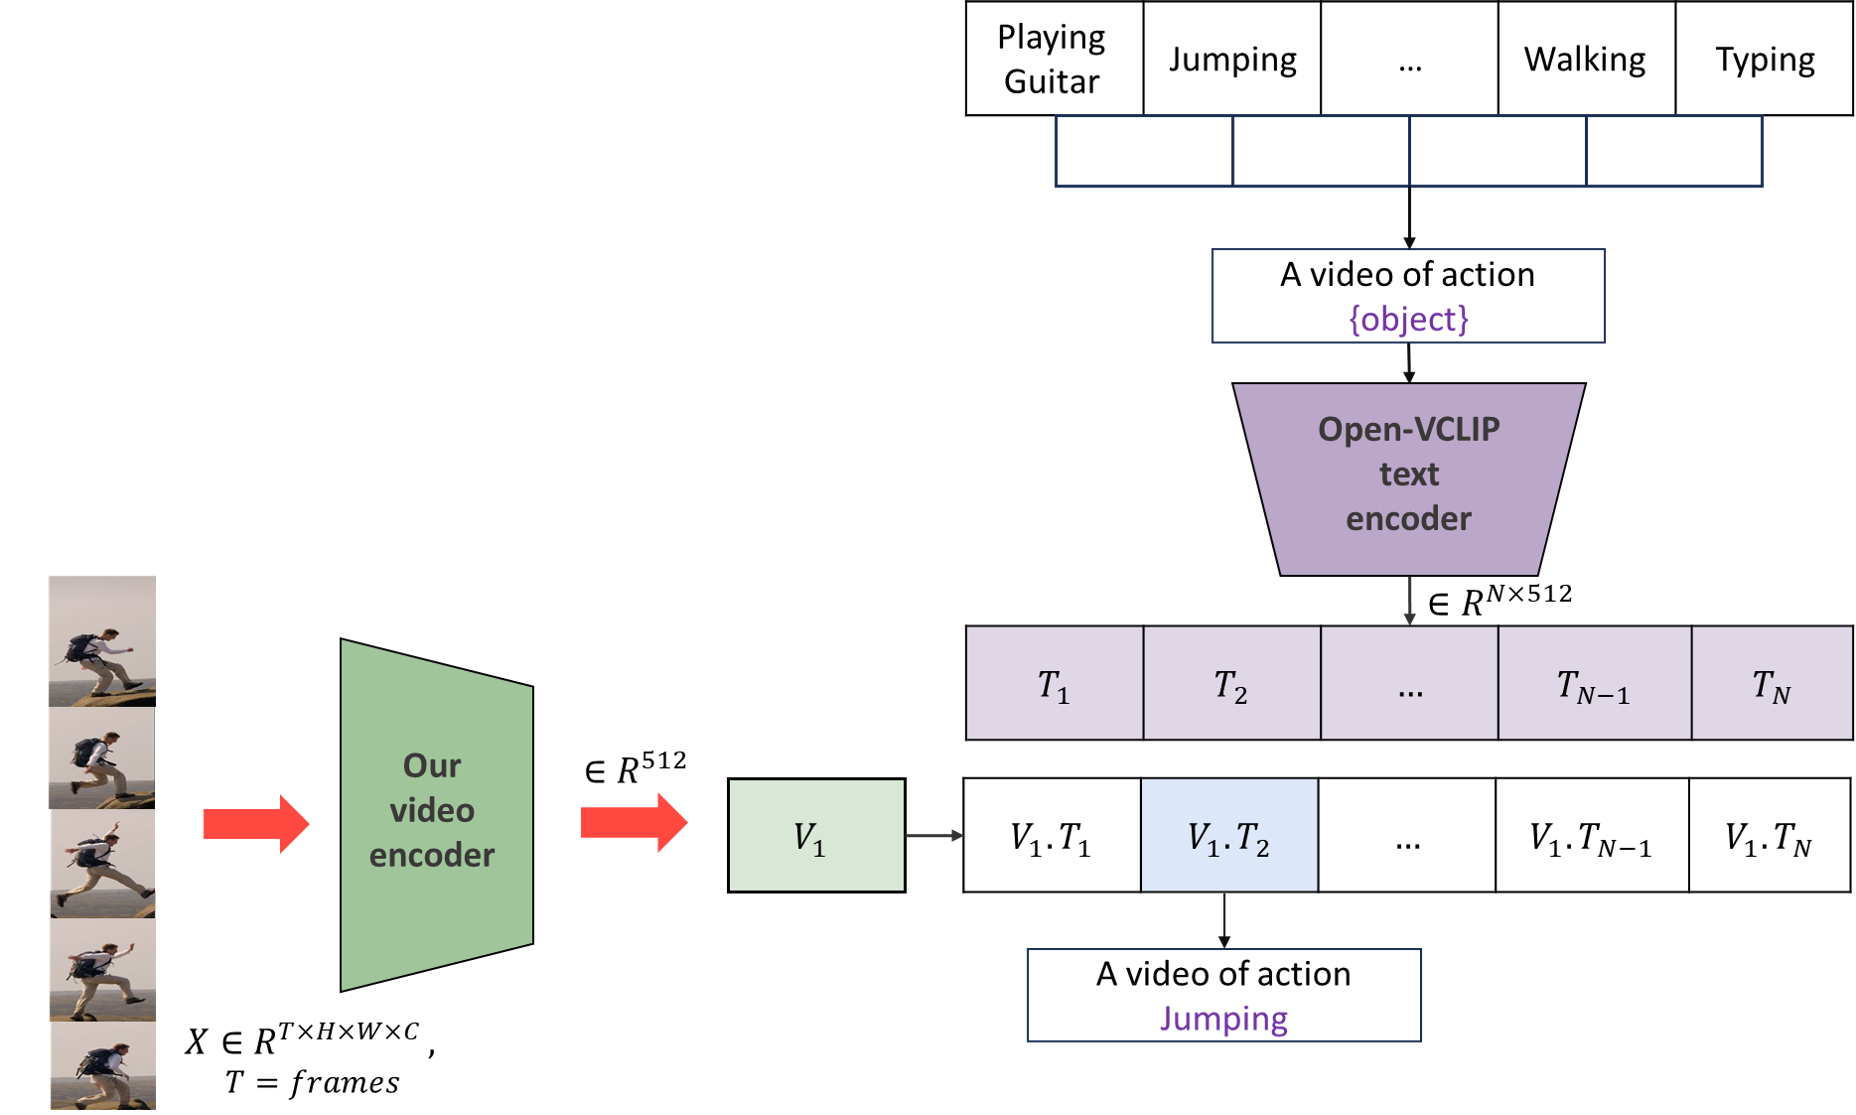
\includegraphics[scale=.48]{Images/Chapter3/test_phase.png}
	\caption[]{طرح کلی مرحله‌ی آزمون مدل \lr{ProActionCLIP}}
	\label{fig.35}
\end{figure}
\section{جمع‌بندی}
در این فصل مدل نهایی پیشنهادی این پژوهش با نام \lr{ProActionCLIP} معرفی شد که ترکیبی از دو مدل \lr{L2P} و \lr{Open-VCLIP} بوده که با تلفیق قابلیت یادگیری پرامپت در \lr{L2P} و توانایی استخراج ویژگی‌های ویدیویی در \lr{Open-VCLIP} طراحی شده است. در این فصل، ساختار کلی مدل پیشنهادی و اجزای اصلی آن شامل کدگذار ویدیو، کدگذار متن منجمد و سازوکار یادگیری پرامپت تشریح شد. تکنیک‌های مختلف استفاده شده در طراحی استخر پرامپت‌ها و روش انتخاب پرامپت‌های مناسب برای هر ورودی، نیز شرح داده شد. همچنین نحوه تعامل این اجزا با یکدیگر برای یادگیری پیوسته و به‌روزرسانی وزن‌های پرامپت‌ها از طریق الگوریتم پس‌انتشار توضیح داده شد. در نهایت، فرآیند آموزش مدل و محاسبه تابع زیان که شامل عبارت منظم‌سازی (برای نزدیک کردن کلیدها و ویژگی ویدیو) و معیار تقابلی است، مورد بررسی قرار گرفت.



\chapter{مشخصات یک پایان نامه و گزارش علمی}

اگرچه براي همه انواع نوشته‌ها، مشخصات و ويژگي‌هاي واحد و معيني نمي‌توان ذكر كرد، با اين حال در یک پایان نامه یا گزارش علمی باید نکات و موارد کلی که در این فصل ذکر می‌شود، بطور کامل رعایت شده باشد. 

دقت كنيد كه پس از عنوان فصل بايد حداقل توضیحی کوتاه در مورد موضوع نوشته شود و نمي‌توان مستقيماً بعد از آن عنوان بخش را نوشت و همين طور پس از عناوين بخش‌ها و زيربخش‌ها.(مانند دستورالعمل حاضر)
\section{برخورداری از غنای علمی }

يك پایان نامه بايد پیش از هر چيز به‌لحاظ علمي از غناي لازم برخوردار باشد. يعني هدف و پيام روشني داشته باشد و از پيش‌زمينه علمي، بيان دلايل علمی، ارجاعات مورد نیاز و نتيجه‌گيري شفاف بهره ببرد. 

\section{ارجاع به‌موقع و صحیح به منابع دیگر}
هر جمله‌ای که در یک پایان نامه نوشته می‌شود یا یک جمله کاملاً بدیهی است یا باید دلیل آن بیان شود و یا اینکه باید به منبعی که آن موضوع را نقل یا اثبات کرده، ارجاع داده شود. اگر مطلب يا گفتاري از منبعی عيناً در گزارش نقل مي‌شود، بايد آن مطلب داخل گيومه قرار گيرد و با ذكر ماخذ و شماره صفحه، به آن اشاره گردد.


\section{ساده‌نویسی }
سادگی از ضروريات يك نوشته است. نويسنده بايد ساده، روان و در عين حال شيوا و رسا بنويسد و عبارات مبهم، جملات پيچيده و كلمات نامأنوس در نوشته خود به‌كار نبرد. اگر چه افراط در اين امر نيز، به شيوايي نوشته صدمه مي‌زند. به‌كارگیری لغات و اصطلاحات دشوار و دور از ذهن و عبارات و جملات نامنظم و مبهم موجب ايجاد اشكال در فهم خواننده خواهد شد‌. 

 براي ساده‌نويسي بايد در حد امكان از به‌كارگيری كلمات «مي‌بايست»، «بايستي»، «گرديد»، «بوده باشد» و مانند آنها كه تكلف‌آور، غلط مصطلح و يا غيرشيوا هستند، به‌جای «بايد»، «است»، «شد» و مثل آنها، اجتناب شود‌.‌ همين‌طور، «در‌جهت» نمی‌تواند جايگزين خوبی برای كلمه روانی مثل «برای» باشد‌. ‌كلمات و جملات روان و ساده مي‌توانند اغلب مفاهيم را براحتی منتقل كنند‌.‌
 
دقت در تنظیم بندها (پاراگراف‌ها) نيز كمك شاياني به روانی و سادگی فهم مطلب مي‌كند‌.‌ بندهای طولانی نيز مانند جملات طولانی مي‌توانند خسته‌كننده باشند و خواننده را سردرگم كنند‌.‌ يك بند نبايد کمتر از سه یا چهار سطر یا بيشتر از $10$ تا 15 سطر باشد.‌ 

\section{وحدت موضوع}

نویسنده بايد در سراسر نوشته از اصل موضوع دور نيافتد و تمام بحث‌ها، مثال‌ها و اجزاي نوشته با هماهنگي كامل، پيرامون موضوع اصلي باشد و تاثيري واحد در ذهن خواننده القا كند. 
\section{اختصار}

پایان نامه یا گزارش علمی بايد در حد امكان، مختصر و مفيد باشد و از بحث‌هاي غير ضروري در آن پرهيز شود. نوشتن مطالب ارزشمندي كه هيچ ربطي به موضوع ندارد، فاقد ارزش علمي است.
\section{رعایت نكات دستوري و نشانه‌گذاري}
در سراسر پایان نامه بايد قواعد دستوري رعايت شود و اركان و اجزاي جمله در جاي مناسب خود آورده شود. همچنین رعايت قواعد نشانه‌گذاري سبب مي‌شود كه بيان نويسنده روشن باشد و خواننده به سهولت و با کمترین صرف انرژی مطالب را مطالعه و درك كند.
\section{توجه به معلومات ذهنی مخاطب}
نويسنده بايد همواره مخاطب خود را در برابر خود تصور كند و با توجه به معلومات ذهني مخاطب  تمامي پیش‌نیازهای لازم براي درك مطالب مورد بحث را، از پیش براي مخاطب فراهم كند.

\section{رعایت مراحل اصولی نگارش}
هر کار علمی زمانی به بهترین شکل قابل انجام است که بر اساس یک برنامه‌ریزی مشخص انجام شود. تهیه یک متن علمي با کیفیت نیز نیازمند برنامه‌ریزی مناسب و اجرای منظم آن می‌باشد. مراحل نگارش را عموماً می‌توان به ترتیب زیر درنظر گرفت:
\begin{itemize}


\item	تهيه فهرستی از عناوین اصلي و فرعی که باید نوشته شود
\item 	اولویت‌بندی و تعیین ترتیب منطقی فصل‌ها و بخش‌های گزارش
\item 	گردآوري اطلاعات اولیه راجع به هر بخش و زیربخش
\item 	تدوین مطالب جدیدی که باید به قلم نگارنده به گزارش اضافه شود
\item 	تایپ كردن مطالب با رعایت کامل نکاتی که در این دستورالعمل آموزش داده می‌شود
\end{itemize}
رعایت نظم و ترتیب در اجرای مراحل ذکر شده هم فرآیند تهیه پایان نامه یا گزارش علمی را برای نگارنده آسان می‌کند و هم کیفیت نگارش را به میزان قابل توجهی افزایش می‌دهد.

















\chapter{جمع‌بندي و نتيجه‌گيري و پیشنهادات}
\label{chap5:concolusion}
%%%%%%%%%%%%%%%%%%%%%%%%%%%%%%%%%%%%%%%%%%%
در این پایان نامه به معرفی مدل پیشنهادی \lr{ProActionCLIP} برای یادگیری پیوسته در داده‌های ویدیویی پرداخته شد. این روش با ترکیب توانایی‌های مدل \lr{Open-VCLIP} در استخراج ویژگی‌های ویدیو و سازوکار پرامپت‌های یادگیرنده در \lr{L2P}، توانسته است بدون تغییر مستقیم پارامترهای مدل پایه‌ی \lr{Open-VCLIP}، به یادگیری پیوسته‌ی وظایف در حوزه‌ی ویدیو بپردازد. به عبارت دیگر، \lr{ProActionCLIP} با بهره‌گیری از مزیت‌های هر دو مدل مرجع، راهکاری مؤثر در یادگیری پیوسته، برای تشخیص حرکت انسان در حوزه‌ی ویدیو ارائه می‌دهد. نتایج حاصل نشان داد که این مدل، ضمن حفظ دانش پیشین و کاهش قابل‌توجه فراموشی فاجعه‌بار، از لحاظ مصرف حافظه و منابع محاسباتی عملکرد بهتری نسبت به سایر روش‌های مشابه داشته است. 
\section{پیشنهادات}
با توجه به نتایج و تحلیل‌های ارائه‌شده، چند مسیر پژوهشی برای بهبود روش پیشنهادی قابل بررسی است:

\begin{enumerate}
	\item \textbf{کاهش شباهت کلیدها بین کلاس‌های مشابه:} 
	یکی از چالش‌های اصلی در افزایش تعداد وظایف، شباهت میان برچسب‌ها است که منجر به شباهت کلیدهای متناظر آن‌ها می‌شود. این امر می‌تواند باعث انتخاب نادرست پرامپت‌ها گردد. پیشنهادی که می‌توان مطرح کرد، در نظر گرفتن یک مؤلفه در تابع زیان است که فاصله‌ی کلیدهای مربوط به برچسب‌های متفاوت را افزایش دهد. به این ترتیب، احتمال شباهت کلیدها بین کلاس‌های نزدیک کاهش یافته و دقت انتخاب پرامپت‌ها بهبود می‌یابد.
	
	\item \textbf{افزایش تعداد پرامپت‌های اختصاصی برای هر کلاس:} 
	اختصاص تعداد بیشتری پرامپت به هر کلاس می‌تواند انعطاف‌پذیری مدل را در یادگیری ویژگی‌های متنوع آن کلاس افزایش دهد و عملکرد کلی سیستم را بهبود بخشد.
\end{enumerate}
\chapter{موارد به‌روزرسانی}
\section{ استفاده از \lr{subfigure}}
برای شکل‌های 
\ref{fig:fig1} و \ref{fig:fig2}
به کد مراجعه نمایید
\begin{figure}[h!]
		\centering % <-- added
		\begin{subfigure}{0.33\textwidth}
			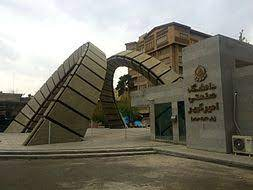
\includegraphics[width=\linewidth]{Images/Chapter6/test1.jpg}
			\caption{\lr{test1}}
			\label{f61}
		\end{subfigure}\hfil % <-- 
		\begin{subfigure}{0.33\textwidth}
			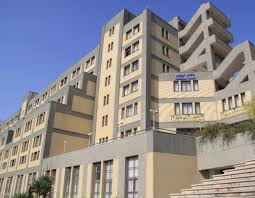
\includegraphics[width=\linewidth]{Images/Chapter6/test2.jpg}
			\caption{\lr{test2}}
			\label{f62}
		\end{subfigure}\hfil % <-- added
        \begin{subfigure}{0.33\textwidth}
			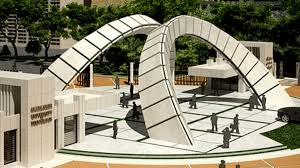
\includegraphics[width=\linewidth]{Images/Chapter6/test3.jpg}
			\caption{\lr{test3}}
			\label{f63}
        \end{subfigure}
		\caption{دانشگاه امیرکبیر}
		\label{fig:fig1}
\end{figure}
 \begin{figure}[ht]
		\centering % <-- added
		\begin{subfigure}{0.45\textwidth}
			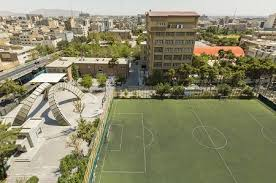
\includegraphics[width=\linewidth, height=0.2\textheight]{Images/Chapter6/test5.jpg}
			\caption{\lr{test5}}
			\label{f64}
		\end{subfigure}\hfil % <-- added
		\begin{subfigure}{0.45\textwidth}
			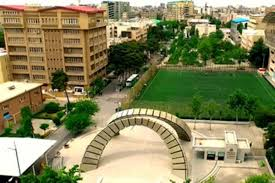
\includegraphics[width=\linewidth, height=0.2\textheight]{Images/Chapter6/test6.jpg}
			\caption{\lr{test6}}
			\label{f65}
		\end{subfigure}
		\caption{پلی تکنبیک}
		\label{fig:fig2}
\end{figure}
\section{فرض}
\begin{asum}
     برای استفاده از فرض کافیست از فرمت زیر استفاده کنید
\begin{latin}
     \normalsize
     \begin{verbatim}
    \begin{asum}
    
    \end{asum}
    \end{verbatim}
\end{latin}
\section{جدول }
\subsection{چندسطری}
مثالی از جدول چند سطری را می‌توانید در \ref{Table1} مشاهده نمایید.
\begin{table}[ht]
    \centering
    \caption{مقایسه الگوریتم‌های بهینه‌ساز}
    \begin{tabular}{|c|c|c|c|} \hline 
        \label{Table1}
        & سناریو & تعداد پارامترها  & تابع هزینه\\  
        \hline
        \multirow{4}{*}{\lr{GWO}} & 1 & 11 & $2.4241$     \\
        & 2 & 8 & $9.1389$           \\
        & 3 & 7 & $6.3343$     \\
        & 4 & 4 & $1.61788$     \\\hline
        \multirow{4}{*}{\lr{PSO}} & 1 & 11 & $20.5801$ \\
        & 2 & 8 & $10.1402$\\
        & 3 & 7 & $3.83659$ \\
        & 4 & 4 & $4.86521$\\\hline
        \multirow{4}{*}{\lr{GA}}  & 1 & 11 & $34.8627$\\
        & 2 & 8 & $33.7109$\\
        & 3 & 7 & $26.4257$\\
        & 4 & 4 & $25.6392$\\\hline						
    \end{tabular}
\end{table}
\end{asum}
\subsection{مقیاس بندی}
برای تنظیم جدول می‌توانید از دستور زیر استفاده نمایید
\begin{latin}
     \normalsize
     \begin{verbatim}
    \adjustbox{max width=\textwidth,max totalheight=\textheight, keepaspectratio}{
    \begin{tabular}...
    .
    .
    .
    \end{tabular}}
    \end{verbatim}
\end{latin}
یا 
\begin{latin}
     \normalsize
     \begin{verbatim}
    \adjustbox{width=\columnwidth,max totalheight=\textheight, keepaspectratio}{
    \begin{tabular}...
    .
    .
    .
    \end{tabular}}
    \end{verbatim}
\end{latin}
نمونه جدول بدون تنظیم
\begin{table}[ht]
    \begin{tabular}{|c|c|c|c|c|c|c|c|c|c|c|c|c|} \hline 
        & $c_1^{\alpha}$ & $c_2^{\alpha}$ & $c_1^{\gamma}$ & $c_2^{\gamma}$ & $d$ & $k$ & $d_{L_2}$ & $d_{L_3}$ & $d_{L_4}$ & $d_{\varepsilon}$ & \lr{SW} & $N$\\  
        \hline
        مثلث  & $6.6$ & $2.4$ & $4.3$ & $11.2$ & $8.6603$ & $1.07$ & $15.3696$ & $24.9362$ & $35.9237$ & $1.5$ & 110 & 58  \\\hline
        پنج شلعی  & $6.1$ & $2.8$ & $4.9$ & $12.7$ & $5.8779$ & $1.09$ & $13.2074$ & $20.6509$ & $29.0499$ & $0.9$ & 75 & 72 \\\hline
        شش ضلعی  & $5.9$ & $2.3$ & $5.2$ & $13.3$ & $5$ & $1.1$& $11.2349$ & $17.5667$ & $23.9169$ & 1 & 70 & 72 \\\hline
    \end{tabular}
    \centering
    \caption{پارامترهای الگوریتم}
    \label{Table2}
\end{table}\\
نمونه جدول با تنظیم سایز
\begin{table}[ht]
\adjustbox{max width=\textwidth,max totalheight=\textheight, keepaspectratio}{%
    \begin{tabular}{|c|c|c|c|c|c|c|c|c|c|c|c|c|} \hline 
        & $c_1^{\alpha}$ & $c_2^{\alpha}$ & $c_1^{\gamma}$ & $c_2^{\gamma}$ & $d$ & $k$ & $d_{L_2}$ & $d_{L_3}$ & $d_{L_4}$ & $d_{\varepsilon}$ & \lr{SW} & $N$\\  
        \hline
        مثلث  & $6.6$ & $2.4$ & $4.3$ & $11.2$ & $8.6603$ & $1.07$ & $15.3696$ & $24.9362$ & $35.9237$ & $1.5$ & 110 & 58  \\\hline
        پنج شلعی  & $6.1$ & $2.8$ & $4.9$ & $12.7$ & $5.8779$ & $1.09$ & $13.2074$ & $20.6509$ & $29.0499$ & $0.9$ & 75 & 72 \\\hline
        شش ضلعی  & $5.9$ & $2.3$ & $5.2$ & $13.3$ & $5$ & $1.1$& $11.2349$ & $17.5667$ & $23.9169$ & 1 & 70 & 72 \\\hline
    \end{tabular}}
    \centering
    \caption{پارامترهای الگوریتم}
    \label{Table3}
\end{table}
\begin{table}[ht]
\adjustbox{width=\columnwidth,max totalheight=\textheight, keepaspectratio}{%
    \begin{tabular}{|c|c|c|c|c|c|c|c|c|c|c|c|c|} \hline 
        & $c_1^{\alpha}$ & $c_2^{\alpha}$ & $c_1^{\gamma}$ & $c_2^{\gamma}$ & $d$ & $k$ & $d_{L_2}$ & $d_{L_3}$ & $d_{L_4}$ & $d_{\varepsilon}$ & \lr{SW} & $N$\\  
        \hline
        مثلث  & $6.6$ & $2.4$ & $4.3$ & $11.2$ & $8.6603$ & $1.07$ & $15.3696$ & $24.9362$ & $35.9237$ & $1.5$ & 110 & 58  \\\hline
        پنج شلعی  & $6.1$ & $2.8$ & $4.9$ & $12.7$ & $5.8779$ & $1.09$ & $13.2074$ & $20.6509$ & $29.0499$ & $0.9$ & 75 & 72 \\\hline
        شش ضلعی  & $5.9$ & $2.3$ & $5.2$ & $13.3$ & $5$ & $1.1$& $11.2349$ & $17.5667$ & $23.9169$ & 1 & 70 & 72 \\\hline
    \end{tabular}}
    \centering
    \caption{پارامترهای الگوریتم}
    \label{Table4}
\end{table}
\subsection{استفاده از قضیه}
\begin{theorem}
تست
\end{theorem}
\begin{proof}
    تست
\end{proof}
برای تغییر کلمه برهان به اثبات، می‌توانید خط 52 در  \lr{commands.tex} را غیر فعال نمایید.
\\
  اشکال هر سطح از  \lr{itemize} را می توانید با مراجعه به
 \lr{commands.tex} تغییر دهید، کامنت‌های مربوطه برای اینکار مشخص شده است (خطوط 44 تا 50).\\
نمونه‌ای از \lr{itemize} چهار سطحی:
\begin{itemize}
    \item تست
    \begin{itemize}
        \item تست
        \begin{itemize}
            \item تست
            \begin{itemize}
                \item تست
            \end{itemize}
        \end{itemize}
    \end{itemize}
\end{itemize}



%--------------------------------------------------------------------------appendix( مراجع و پیوست ها)
\chapterfont{\vspace*{-2em}\centering\LARGE}%

\appendix
\bibliographystyle{unsrt-fa}
\bibliography{references}
%\chapter*{‌پیوست}
\markboth{پیوست}{}
\addcontentsline{toc}{chapter}{پیوست}
موضوعات مرتبط با متن گزارش پایان نامه كه در يكی از گروه‌های زير قرار می‌گيرد، در بخش پيوست‌ها آورده شوند:
\begin{enumerate}
\item  اثبات های رياضی يا عمليات رياضی طولانی‌.‌
\item داده و اطلاعات نمونه (های) مورد مطالعه (\lr{Case Study}) چنانچه طولانی باشد‌.‌
\item نتايج كارهای ديگران چنانچه نياز به تفصيل باشد‌.‌
\item مجموعه تعاريف متغيرها و پارامترها، چنانچه طولانی بوده و در متن به انجام نرسيده باشد‌.‌
\end{enumerate}
% براي شماره‌گذاري روابط، جداول و اشكال موجود در پيوست‌ از ساختار متفاوتي نسبت به متن اصلي استفاده مي‌شود كه در زير به‌عنوان نمونه نمايش داده شده‌است. 
% \begin{equation}
%F=ma
%\end{equation}
\section*{کد میپل }
\begin{latin}
\begin{verbatim}

with(DifferentialGeometry):
with(Tensor):
DGsetup([x, y, z], M)
																	frame name: M
a := evalDG(D_x)
																	D_x
b := evalDG(-2 y z D_x+2 x D_y/z^3-D_z/z^2)


\end{verbatim}
\end{latin}
%--------------------------------------------------------------------------dictionary(واژه نامه ها)
%اگر مایل به داشتن صفحه واژه‌نامه نیستید، خط زیر را غیر فعال کنید.
\parindent=0pt
%%
\chapter*{واژه‌نامه‌ی فارسی به انگلیسی}
\pagestyle{style9}

\addcontentsline{toc}{chapter}{واژه‌نامه‌ی فارسی به انگلیسی}
%%%%%%
\begin{multicols*}{2}

{\bf آ}
\vspace*{3mm}


\farsiTOenglish{اسکالر}{Scalar}


\vspace*{3mm}
{\bf ب}
\vspace*{3mm}

\farsiTOenglish{بالابر}{Lift}


\vspace*{3mm}
{\bf پ}
%%\vspace*{3mm}

\farsiTOenglish{پایا}{Invariant}



\vspace*{3mm}
{\bf ت}
%%\vspace*{3mm}

\farsiTOenglish{ تناظر }{Correspondence}


\vspace*{3mm}
{\bf ث}
%%\vspace*{3mm}

\farsiTOenglish{ثابت‌ساز}{Stabilizer}

\vspace*{3mm}
{\bf ج}
%%\vspace*{3mm}

\farsiTOenglish{جایگشت}{Permutation}



\vspace*{3mm}
{\bf چ}
%%\vspace*{3mm}


\farsiTOenglish{چند جمله‌ای }{Polynomial}

\vspace*{3mm}
{\bf ح}
%%\vspace*{3mm}

\farsiTOenglish{حاصل‌ضرب دکارتی}{Cartesian product}


\vspace*{3mm}
{\bf خ}
%%\vspace*{3mm}

\farsiTOenglish{خودریختی}{Automorphism}

\vspace*{3mm}
{\bf د}
%%\vspace*{3mm}

\farsiTOenglish{درجه}{Degree}


\vspace*{3mm}
{\bf ر}
%%\vspace*{3mm}


\farsiTOenglish{ریزپردازنده}{microprocessor}


\vspace*{3mm}
{\bf ز}
%%\vspace*{3mm}


\farsiTOenglish{زیرمدول}{Submodule}


\vspace*{3mm}
{\bf س}
%%\vspace*{3mm}

\farsiTOenglish{سرشت}{Character}


\vspace*{3mm}
{\bf ص}
%%\vspace*{3mm}

\farsiTOenglish{صادقانه}{Faithful}

\vspace*{3mm}
{\bf ض}
%%\vspace*{3mm}

\farsiTOenglish{ضرب داخلی}{Inner product}

\vspace*{3mm}
{\bf ط}
%%\vspace*{3mm}


\farsiTOenglish{طوقه}{Loop}


\vspace*{3mm}
{\bf ظ}
%%\vspace*{3mm}


\farsiTOenglish{ظرفیت}{Valency}
 
\vspace*{3mm}
{\bf ع}
%%\vspace*{3mm}


\farsiTOenglish{عدم مجاورت}{Nonadjacency}



\vspace*{3mm}
{\bf ف}
%%\vspace*{3mm}

\farsiTOenglish{فضای برداری}{Vector space}



\vspace*{3mm}
{\bf ک}
%%\vspace*{3mm}

\farsiTOenglish{کاملاً تحویل‌پذیر}{Complete reducibility}


\vspace*{3mm}
{\bf گ}
%%\vspace*{3mm}


\farsiTOenglish{گراف}{Graph}



\vspace*{3mm}
{\bf م}
%%\vspace*{3mm}

\farsiTOenglish{ماتریس جایگشتی}{Permutation matrix }


\vspace*{3mm}
{\bf ن}
%%\vspace*{3mm}

\farsiTOenglish{ناهمبند}{Disconnected}


\vspace*{3mm}
{\bf و}
%%\vspace*{3mm}

\farsiTOenglish{وارون‌پذیر}{Invertible}


\vspace*{3mm}
{\bf ه}
%%\vspace*{3mm}

\farsiTOenglish{همبند}{Connected}



\vspace*{3mm}
{\bf ی}
%%\vspace*{3mm}

\farsiTOenglish{یال}{Edge}




\end{multicols*}%
%%%%%%%
\chapter*{ واژه‌نامه‌ی انگلیسی به فارسی}
\pagestyle{style9}
\lhead{\thepage}\rhead{واژه‌نامه‌ی انگلیسی به فارسی}
\addcontentsline{toc}{chapter}{واژه‌نامه‌ی انگلیسی به فارسی}

\LTRmulticolcolumns
\begin{multicols}{2}
{\hfill\bf  \lr{A}}
%%\vspace*{1.5mm}

\englishTOfarsi{Automorphism}{خودریختی}

\vspace*{3mm}
{\hfill\bf   \lr{B}}
%%\vspace*{1.5mm}

\englishTOfarsi{Bijection}{دوسویی}

\vspace*{3mm}
{\hfill\bf   \lr{C}}
%%\vspace*{1.5mm}

\englishTOfarsi{Cycle group}{گروه دوری}

\vspace*{3mm}
{\hfill\bf   \lr{D}}
%%\vspace*{1.5mm}

\englishTOfarsi{Degree}{درجه}

\vspace*{3mm}
{\hfill\bf   \lr{E}}
%%\vspace*{1.5mm}

\englishTOfarsi{Edge}{یال}

\vspace*{3mm}
{\hfill\bf   \lr{F}}
%%\vspace*{1.5mm}

\englishTOfarsi{Function}{تابع}

\vspace*{3mm}
{\hfill\bf   \lr{G}}
%%\vspace*{1.5mm}

\englishTOfarsi{Group}{گروه}

\vspace*{3mm}
{\hfill\bf   \lr{H}}
%%\vspace*{1.5mm}

\englishTOfarsi{Homomorphism}{همریختی}

\vspace*{3mm}
{\hfill\bf   \lr{I}}
%%\vspace*{1.5mm}

\englishTOfarsi{Invariant}{پایا}

\vspace*{3mm}
{\hfill\bf   \lr{L}}
%%\vspace*{1.5mm}

\englishTOfarsi{Lift}{بالابر}

\vspace*{3mm}
{\hfill\bf   \lr{M}}
%%\vspace*{1.5mm}

\englishTOfarsi{Module}{مدول}

\vspace*{3mm}
{\hfill\bf   \lr{N}}
%%\vspace*{1.5mm}

\englishTOfarsi{Natural map}{نگاشت طبیعی}

\vspace*{3mm}
{\hfill\bf   \lr{O}}
%%\vspace*{1.5mm}

\englishTOfarsi{One to One}{یک به یک}

\vspace*{3mm}
{\hfill\bf   \lr{P}}
%%\vspace*{1.5mm}

\englishTOfarsi{Permutation group}{گروه جایگشتی}

\vspace*{3mm}
{\hfill\bf   \lr{Q}}
%%\vspace*{1.5mm}

\englishTOfarsi{Quotient graph}{گراف خارج‌قسمتی}

 \vspace*{3mm}
{\hfill\bf   \lr{R}}
%%\vspace*{1.5mm}

\englishTOfarsi{Reducible}{تحویل پذیر}

\vspace*{3mm}
{\hfill\bf   \lr{S}}
%%\vspace*{1.5mm}

\englishTOfarsi{Sequence}{دنباله}

 \vspace*{3mm}
{\hfill\bf   \lr{T}}
%%\vspace*{1.5mm}

\englishTOfarsi{Trivial character}{سرشت بدیهی}

\vspace*{3mm}
{\hfill\bf   \lr{U}}
%%\vspace*{1.5mm}

\englishTOfarsi{Unique}{منحصربفرد}

\vspace*{3mm}
{\hfill\bf   \lr{V}}
%%\vspace*{1.5mm}

\englishTOfarsi{Vector space}{فضای برداری}
\end{multicols}
%--------------------------------------------------------------------------index(نمایه)
%اگر مایل به داشتن صفحه نمایه نیستید، خط زیر را غیر فعال کنید.
\pagestyle{style7}
\printindex
\pagestyle{style7}
%%کلمات کلیدی انگلیسی
\latinkeywords{Write a 3 to 5 KeyWords is essential. Example: AUT, M.Sc., Ph. D,..}
%چکیده انگلیسی

\en-abstract{
In recent years, machine learning—and in particular, deep neural networks—have made remarkable advancements, achieving near-human performance in fields such as computer vision, natural language processing, and speech recognition. Achieving such performance typically requires pre-training these networks on large-scale datasets, a process that enables the reuse of trained models across a variety of tasks. In many real-world applications, however, data becomes available incrementally and in the form of sequential tasks, highlighting the need for continual learning approaches. A major challenge in this domain is catastrophic forgetting, wherein the model suffers a significant drop in performance on previously learned tasks after acquiring new ones. Despite recent developments in large language models and vision-language models, limitations such as high memory consumption remain. This research introduces ProActionCLIP, a method for continual learning on video data that combines the feature extraction capabilities of the vision-language model Open-VCLIP with the learnable prompt mechanism from the L2P model. This integration enables adaptation to sequential tasks without altering the main parameters of the base Open-VCLIP model, while optimizing prompt selection to mitigate catastrophic forgetting. Experimental results demonstrate that the proposed method not only preserves prior knowledge and effectively learns new knowledge, but also offers high efficiency in terms of memory and computational resource usage. Consequently, it provides an effective solution for continual learning in human action recognition within video datasets.
}
%%%%%%%%%%%%%%%%%%%%% کدهای زیر را تغییر ندهید.

\newpage
\thispagestyle{empty}
\begin{latin}
\section*{\LARGE\centering Abstract}

\een-abstract

\vspace*{.5cm}
{\large\textbf{Keywords:}}\par
\vspace*{.5cm}
Continual learning, vision-language model, prompt learning, catastrophic forgetting
\end{latin}
% در این فایل، عنوان پایان‌نامه، مشخصات خود و چکیده پایان‌نامه را به انگلیسی، وارد کنید.
%%%%%%%%%%%%%%%%%%%%%%%%%%%%%%%%%%%%
\baselineskip=.6cm
\begin{latin}

\latinfaculty{Department of ...}


\latintitle{Title of Thesis}


\firstlatinsupervisor{Dr. }

%\secondlatinsupervisor{Second Supervisor}

\firstlatinadvisor{Dr. }

%\secondlatinadvisor{Second Advisor}

\latinname{Name}

\latinsurname{Surname}

\latinthesisdate{Month \& Year}

\latinvtitle
\end{latin}

\end{document}